\documentclass[letterpaper,12pt]{article}
\usepackage{tabularx} % extra features for tabular environment
\usepackage{amsmath}  % improve math presentation
\usepackage{amssymb}
\usepackage{graphicx} % takes care of graphic including machinery
\usepackage[margin=1in,letterpaper]{geometry} % decreases margins
\usepackage{cite} % takes care of citations
\usepackage{mathtools} % for defining KL divergence command
\usepackage[margin=1in]{geometry} % make margins smaller
\usepackage[ruled,lined]{algorithm2e} % takes care of algorithms
\DontPrintSemicolon % don't print semicolon in algorithms
\usepackage{verbatim} % for block commenting
\usepackage{subcaption} % for sub-figures
\usepackage{biblatex} % for bibliography
\addbibresource{bibliography.bib} % import bibliography file
\usepackage[final]{hyperref} % adds hyper links inside the generated pdf file
\hypersetup{
	colorlinks=true,       % false: boxed links; true: colored links
	linkcolor=blue,        % color of internal links
	citecolor=blue,        % color of links to bibliography
	filecolor=magenta,     % color of file links
	urlcolor=blue         
}
\usepackage{blindtext}
%++++++++++++++++++++++++++++++++++++++++
% miscellaneous commands
\newcommand{\R}{\mathbb{R}} % real number R
\newcommand{\PP}{\mathbb{P}} % fancy probability 'p'
\newcommand{\B}[1]{\mathbf{#1}} % to make a number bold

% brackets, braces, and parenthesis
\newcommand{\lc}{\left \{} % left curly bracket
\newcommand{\rc}{\right \}} % right curly bracket
\newcommand{\lp}{\left (} % left parenthesis
\newcommand{\rp}{\right )} % right parenthesis
\newcommand{\lb}{\left [} % left bracket
\newcommand{\rb}{\right ]} % right bracket

% commands for PDF p in terms of x and z
\newcommand{\px}{\ensuremath{p(\boldsymbol{x})}}
\newcommand{\pz}{\ensuremath{p(\boldsymbol{z})}}
\newcommand{\pzx}{\ensuremath{p(\boldsymbol{z}, \boldsymbol{x})}}
\newcommand{\pzgivenx}{\ensuremath{p(\boldsymbol{z} | \boldsymbol{x})}}
\newcommand{\pxgivenz}{\ensuremath{p(\boldsymbol{x} | \boldsymbol{z})}}

% commands for PDF q in terms of x and z
\newcommand{\qx}{\ensuremath{q(\boldsymbol{x})}}
\newcommand{\qz}{\ensuremath{q(\boldsymbol{z})}}
\newcommand{\qzx}{\ensuremath{q(\boldsymbol{z}, \boldsymbol{x})}}
\newcommand{\qxgivenz}{\ensuremath{q(\boldsymbol{x} | \boldsymbol{z})}}
\newcommand{\qzgivenx}{\ensuremath{q(\boldsymbol{z} | \boldsymbol{x})}}

%+++++++++++++++++++++++++++++++++++++++++++++++++++++
%  LINEAR MODEL COMMANDS FOR VECTORS AND SCALARS

% commands w/ the variables for our linear model
\newcommand{\sigmaepsilon}{\sigma_\epsilon^2} % sigma epsilon
\newcommand{\mean}[1]{\ensuremath{\boldsymbol{\mu}_{#1}}} % mean vector with input subscript
\newcommand{\rvec}[1]{\ensuremath{\boldsymbol{r}_{#1}}} % r vector with input subscript

\newcommand{\nuv}{\boldsymbol{\nu}} % nu vector
\newcommand{\gammav}{\boldsymbol{\gamma}} % gamma vector

\newcommand{\ti}{\boldsymbol{t}_i} % t_i vector
\newcommand{\ri}{\boldsymbol{r}_i} % r_i vector

\newcommand{\ytilde}{\ensuremath{\tilde{y}}} % y tilde
\newcommand{\ttilde}{\ensuremath{\tilde{\boldsymbol{t}}}} % t tilde vector 
\newcommand{\rtilde}{\ensuremath{\tilde{\boldsymbol{r}}}} % r tilde vector

% commands for mean and covariance parameters of p
\newcommand{\meannu}{\ensuremath{\boldsymbol{\mu_\nuv}}} % mean vector of nu
\newcommand{\meangamma}{\ensuremath{\boldsymbol{\mu_\gammav}}} % mean vector of nu
\newcommand{\Sigmanu}{\Sigma_{\nuv}} % sigma nu covariance matrix
\newcommand{\Sigmagamma}{\Sigma_{\gammav}} % sigma gamma covariance matrix

% commands for mean and covariance parameters of q
\newcommand{\mnu}{\ensuremath{m_\nuv}} % m_nu, the mean of our approximation q(nu)
\newcommand{\snu}{\ensuremath{s_\nuv}} % s_nu, the covariance of our approximation q(nu)
\newcommand{\mgamma}{m_\gammav} % m_gamma, the mean of our approximation q(gamma)
\newcommand{\sgamma}{\ensuremath{s_\gammav}} % s_gamma, the covariance of our approximation q(gamma)

% commands for PDF p in terms of our linear models
\newcommand{\pygiven}{\ensuremath{p(y_i | \nu, \gamma)}}

% commands for PDF q in terms of our linear models
\newcommand{\qtheta}{\ensuremath{q(\boldsymbol{\nu}_\theta})}
\newcommand{\qgammatheta}{\ensuremath{q(\boldsymbol{\gamma}_\theta})}

%+++++++++++++++++++++++++++++++++++++++++++++++++++++
% LINEAR MODEL COMMANDS FOR VECTOR INDEXING FOR nu, THE MEAN OF nu, ti, AND t tilde

% indexing with a
\newcommand{\nua}{\ensuremath{\nuv_a}} % nu vector element a
\newcommand{\tatilde}{\ensuremath{\ttilde_a}} % t tilde vector element a
\newcommand{\nuaprime}{\ensuremath{\nuv_{a'}}} % nu vector element a prime
\newcommand{\taprimetilde}{\ensuremath{\ttilde_{a'}}} % t tilde vector element a prime
\newcommand{\meananu}{\ensuremath{\boldsymbol{\mu_{\nuv_a}}}} % mean vector of nu indexed by a
\newcommand{\meanaprimenu}{\ensuremath{\boldsymbol{\mu_{\nuv_{a'}}}}} % mean vector of nu indexed by a'
\newcommand{\tia}{\ensuremath{\boldsymbol{t}_{i_a}}} % ti vector indexed by a
\newcommand{\tiaprime}{\ensuremath{\boldsymbol{t}_{i_{a'}}}} % ti vector indexed by a'
\newcommand{\rbtilde}{\ensuremath{\rtilde_b}} % t tilde vector element a
\newcommand{\rib}{\ensuremath{\boldsymbol{r}_{i_b}}} % ri vector indexed by b
\newcommand{\ribprime}{\ensuremath{\boldsymbol{r}_{i_{b'}}}} % ri vector indexed by b'

% indexing with theta
\newcommand{\tthetatilde}{\ensuremath{\boldsymbol{t}_{i_\theta}}} % t tilde vector element theta
\newcommand{\nutheta}{\ensuremath{\nuv_\theta}} % nu vector element theta
\newcommand{\meannutheta}{\ensuremath{\boldsymbol{\mu_{\nuv_\theta}}}} % mean vector of nu indexed by theta
\newcommand{\sigmanutheta}{\ensuremath{\Sigma_{\nuv_{\theta, \theta}}}}
\newcommand{\meangammatheta}{\ensuremath{\boldsymbol{\mu_{\gammav_\theta}}}} % mean vector of gamma indexed by theta

% commands for mean and covariance parameters of q
\newcommand{\mnusub}[1]{\ensuremath{m_{\nuv_#1}}} % m_nu, the mean of our approximation q(nu)
\newcommand{\snusub}[1]{\ensuremath{s_{\nuv_#1}}} % s_nu, the covariance of our approximation q(nu)
\newcommand{\mgammasub}[1]{\ensuremath{m_{\gammav_#1}}} % m_gamma, the mean of our approximation q(gamma)
\newcommand{\sgammasub}[1]{\ensuremath{s_{\gammav_#1}}} % s_gamma, the covariance of our approximation q(nu)

%++++++++++++++++++++++++++++++++++++++++++++++++

% commands for vectors
\newcommand{\x}{\mathbf{x}}
\newcommand{\z}{\mathbf{z}}

% command for KL divergence
\DeclarePairedDelimiterX{\infdivx}[2]{(}{)}{%
  #1\;\delimsize|\delimsize|\;#2%
}
\newcommand{\kld}[2]{\ensuremath{\mathrm{KL}\infdivx{#1}{#2}}\xspace}

% command for ELBO
\newcommand{\elboq}{\ensuremath{\mathrm{ELBO}(q)}}
\newcommand{\elbo}{\ensuremath{\mathrm{ELBO}}}

% command for CAVI
\newcommand{\cavi}{\ensuremath{\mathrm{CAVI}}}

% commands for expectation
\newcommand{\E}{\mathbb{E}_q}
\newcommand{\Etheta}{\ensuremath{\mathbb{E}_{q_{-\theta}}}} % expectation w.r.t. negative theta
\newcommand{\el}{\left[} % expectation left bracket
\newcommand{\er}{\right]} % expectation right bracket

% settings for algorithm
\SetKwInput{KwInput}{Input}                % Set the Input
\SetKwInput{KwOutput}{Output}              % set the Output
\SetKwInput{KwInitialize}{Initialize}       % Set the initialization
%++++++++++++++++++++++++++++++++++++++++
\DeclareMathOperator*{\argmin}{arg\,min}

\begin{document}

\title{Simulating Variational Approximations of $\alpha$-Posteriors}
\author{Gilead Turok}
\date{\today}
\maketitle

\begin{abstract}
    Previous work has suggested that in misspecified models, $\alpha$-posteriors and their variational approximations are more robust than their standard counterparts. I examine this theory empirically with a simple, linear model. I derive the $\cavi_\alpha$ algorithm for its variational approximation, both when the model is properly specified and when it is misspecified. I then simulate these models and demonstrate that what works in theory, also works in practice.
\end{abstract}


\section{Introduction}
\subsection{Variational Inference}

\textbf{Why Approximations Are Necessary} One of the most important areas of research in modern statistics is approximating difficult-to-compute probability densities in Bayesian statistics or for other complex models. But what makes them so hard to compute? To explain, consider a joint density $\pzx$ that serves as a model for observations $\x=x_{1:n}$ and latent variables $\z=z_{1:m}$. From a Bayesian perspective, we often care about computing $\pzgivenx$, the posterior density:

\begin{equation*}
    \pzgivenx = \frac{\pzx}{\px} = \frac{\pzx}{\int \pzx d\z}
\end{equation*}

When calculating the evidence \px, its integral is often unavailable in closed form or requires exponential time to compute, making the posterior density ultimately infeasible to calculate. To get around this, statisticians have developed alternative methods to approximate $\pzgivenx$. 

\textbf{Approximation Methods} The most popular technique for approximating densities is Markov Chain Monte Carlo (MCMC) sampling. However, MCMC is very slow, making it impractical to use on larger datasets or complex models. Variational Inference (VI) solves these issues, treating the approximation of $\pzgivenx$ as an optimization problem instead of a sampling problem. This allows statisticians to use an entire suite of well-studied optimization techniques that are much faster. VI is less studied than MCMC and is well summarized in \cite{blei}.

\textbf{KL Divergence} To set up the optimization problem of VI, let $\mathcal{Q}$ be a family of densities over the latent variables $\z$. Furthermore, let $q(\z) \in \mathcal{Q}$ be a candidate approximation to the exact conditional. We then use KL divergence -- a distance metric for probability densities -- to measure how good a given approximation is. The optimization problem then becomes selecting the $\qz$ that best minimizes the divergence from \pzgivenx, the true posterior based on the model $\pzx$: 

\begin{equation}
q^*(\z) = \argmin_{\qz \in \mathcal{Q}} \kld{\qz}{\pzgivenx}
\end{equation}

where $q^*(\cdot)$ is the best approximation to $\pzgivenx$ in the approximating set $\mathcal{Q}$.

\textbf{Evidence Lower Bound (ELBO)} However, in this setting, computing the KL divergence is intractable because it actually relies on \px. To see this, recall the definition of KL divergence:
\begin{equation} \label{eq:kl def}
\begin{split}
    \kld{\qz}{\pzgivenx} &= \E \left[\log \qz \right] - \E \left[ \log \pzgivenx \right]\\
    &= \E \left[ \log \qz \right] - \E \left[ \log \pzx \right] + \log \px
\end{split}
\end{equation}

To get around this, we optimize the Evidence Lower Bound (\elbo) which is equivalent to KL up to an added constant. We define it as: 

\begin{equation} \label{eq:elbo def}
    \elboq =\E\left[ \log \pzx \right] - \E \left[ \log \qz \right]
\end{equation}
\noindent Notice how the $\elbo$ is related to KL divergence:
\begin{equation}
\begin{split}
    \elboq &= \E \el \log \pz \er + \E \el \log \pxgivenz \er - \E \el \log \qz \er\\
    &= \E \el \log \pxgivenz \er - \kld{\qz}{\pz}
\end{split}
\end{equation}

\noindent From this we see that minimizing the KL divergence is equivalent to maximizing the $\elbo$ with a constant. Therefore, using the \elbo, our optimization problem now becomes tractable.

Additionally, notice that from \autoref{eq:kl def} and \autoref{eq:elbo def} that

\begin{equation}
    \log \px = \kld{\qz}{\pzgivenx} + \elboq
\end{equation}
Therefore, because $KL(\cdot) \geq 0$, we know that

\begin{equation}
    \log \px \geq \elboq
\end{equation}

\noindent This is how the $\elbo$ gets its name, because it is the lower bound for the evidence, $\log \px$.

\textbf{Mean-Field Variational Family} Choosing $\mathcal{Q}$, the family of possible approximations, is extremely important in managing the complexity of our problem. If $\mathcal{Q}$ is large, it can better capture \pzgivenx, but poses a more difficult optimization problem. If $\mathcal{Q}$ is small, it doesn't capture $\pzgivenx$ as well, but is simpler to optimize.

In this paper, we will use the commonly-used mean-field variational family, which strikes a balanced trade-off between expressiveness and solvability. In this family, $\qz$ is assumed to factorize over the latent variables:

\begin{equation}
    \qz = \prod_{j=1}^m q_j(\B{z}_j)
\end{equation}


Each latent variable is given its own parameter $z_j$ which dictates its density $q_j(z_j)$. To maximize the $\elbo$, therefore, we seek to find the best value of $z_j$. Crucially, the mean-field variational family does not place any restrictions on the nature of the density $q_j(\B{z}_j)$.

\textbf{Coordinate Ascent Variational Inference (CAVI)}
To solve this optimization problem, we use coordinate ascent in an algorithm called CAVI. Note that this optimization procedure, coordinate ascent, is often known as coordinate descent, but because we're searching the maximum, not minimum, we use coordinate ascent instead. This procedure works by optimizing one dimension at a time while holding the remaining dimensions constant. This simplifies the problem, allowing us to climb to the optimum.

Mathematically, it is expressed as

\begin{equation}
\begin{split}
    \log q_j(z_j) &\propto \mathbb{E}_{q_{-j}} \el \log \pzx \er
\end{split}
\end{equation}
    
and is derived in Appendix A. \cite{mao} \cite{zuo}

This gives us the following CAVI algorithm, based off of David Blei's overview of Variational Inference \cite{blei}:

\begin{algorithm}
\KwIn{A model $\pzx$, a data set $\x$}
\KwOut {A variational density $\qz = \prod_{j=1}^m q_j(z_j)$}
\textbf{Initialize:} Variational factors $q_j(z_j)$

\While{the $\elbo$ has not converged}{
    \For {$j \in \{1, \ldots, m \}$} {
        Set $\log q_j(z_j) \propto  \mathbb{E}_{q_{-j}} \el \log \pzx \er$
    }
    Compute $\elboq = \E \el \log \pz \er + \E \el \log \pxgivenz \er - \E \el \log \qz \er$
}
\caption{Coordinate Ascent Variational Inference (CAVI)}
\label{algo:cavi}
\end{algorithm}

\subsection{$\alpha$-Posteriers}

\textbf{Specified and Misspecified Models} When creating statistical models, the underlying modelling assumptions may be correct or may be flawed. If the model is, in fact, correct, I call this a \textit{specified model} and if the model is incorrect, I call this a \textit{misspecified model}.

\textbf{Defining $\alpha$-Posteriors}
The $\alpha$-posterior (also called fractional, tempered, or power posterior) is used in the setting of misspecified models, trying to improve their \textit{robustness}, where robustness (in this context) is defined in terms of a smaller KL divergence to the true model. More specifically, $\alpha$-posteriors raise the likelihood term to the power of $\alpha$. This allows us to compute the posterior as

\begin{equation}
    p(\z|\x; \alpha) = \frac{p(x|z)^\alpha p(z)}{\int p(x|z)^\alpha p(z) d\z}
\end{equation}

Raising the likelihood to the power of $\alpha$ downweights it. 
In variational inference, $\alpha$-posteriors are sometimes used, especially because our latent approximations $q$ are almost always misspecified models.

\textbf{Related Work} Rush \cite{rush} has applied $\alpha$-posteriors to variational inference settings with some insightful results. Firstly, the expected KL divergence between an $\alpha$-posterior and the true posterior is minimized for some $\alpha^* \in [0,1]$. Second, the expected KL divergence between the true posterior and the mean-field variational approximation to the $\alpha$-posterior is also minimized for some $\alpha^* \in [0,1]$; this result suggests that for model misspecification, variational approximations of $\alpha$-posteriors are more robust than variational approximations of regular posteriors.

\textbf{My Work} In this paper, I investigate the above claim empirically. To do this, I first derive an $\elbo_\alpha$ expression and a slightly modified CAVI algorithm. Then, I apply this VI machinery to an extremely simple case of a linear model. Then, I code up these results and examine their performance through a variety of metrics.

\section{The Alpha-CAVI Algorithm}

Recall that one way of expressing the $\elbo$ is 

\begin{equation}
\begin{split}
    \elboq &= \E \el \log \pz \er +  \E \el \log \pxgivenz \er - \E \el \log \qz \er\\
\end{split}
\end{equation}

We define the $\elbo_\alpha$ similarly

\begin{equation}
\begin{split}
    \elbo_\alpha(q) &= \E \el \log \pz \er +  \E \el \log \pxgivenz^\alpha \er  - \E \el \log \qz \er\\
\end{split}
\end{equation}

Now, from Appendix B, we get the coordinate-ascent update as

\begin{equation}
    \log q_j(z_j) \propto \mathbb{E}_{q_{-j}} \el \log \pz \pxgivenz^\alpha \er
\end{equation}

Now the $\cavi_\alpha$ algorithm is

\begin{algorithm}[H]
\KwIn{A model $\pzx$, a data set $\x$}
\KwOut {A variational density $\qz = \prod_{j=1}^m q_j(z_j)$}
\textbf{Initialize:} Variational factors $q_j(z_j)$

\While{the $\elbo_\alpha$ has not converged}{
    \For {$j \in \{1, \ldots, m \}$} {
        Set $\log q_j(z_j) \propto \mathbb{E}_{q_{-j}} \el \log \pz \pxgivenz^\alpha \er$
    }
    Compute $\elbo_\alpha(q) &= \E \el \log \pz \er +  \E \el \log \pxgivenz^\alpha \er  - \E \el \log \qz \er$
}
\caption{Alpha Coordinate Ascent Variational Inference ($\cavi_\alpha$)}
\label{algo:cavi}
\end{algorithm}


\section{Linear Models}
To explore the $\cavi_\alpha$ algorithm, we consider a simple, linear example. Assume that the true, specified model is given by

\begin{equation}
    y_i=\mathbf{\nu}^T\mathbf{t}_i+\mathbf{\gamma}^T \mathbf{r_i}+\epsilon_i \qquad \text{for }i=1\ldots N 
\end{equation}

and the missspecified model, which drops the $\gammav^T \ri$ term, is given by

\begin{equation}
    y_i=\mathbf{\nu}^T\mathbf{t}_i+\epsilon_i \qquad \text{for }i=1\ldots N 
\end{equation}

In this setting, $y_i$ is our observed data, $\lc \nuv, \gammav \rc$ are our latent variables, $\lc \ti, \ri \rc$ are other available data, and $\epsilon_i$ is our noise.

More specifically, $\ti, \ri \sim (0, \mathbb{I})$ and $\epsilon_i \sim \mathcal{N}(0, \sigmaepsilon)$. To make the math a little simpler, we also assume $\nuv \sim \mathcal{N}(\mu_{\nu}, \beta_\nu \mathbb{I})$ and $\gammav \sim \mathcal{N}(\mu_{\gamma}, \beta_\gamma \mathbb{I})$ with $\nuv \in \R^A$ and $\gammav \in \R^B$. Furthermore, let $\mu_\nu, \mu_\gamma \sim U[1,10]$ and $\beta_\nu, \beta_\gamma \sim U[0,1]$.


Furthermore, we will be approximating our latent variables $\nu$ and $\gamma$ with the mean field family of distributions $q$:
\begin{equation}
    q(\nu, \gamma) = q(\nu; m_\nu, s_\nu)q(\gamma; m_\gamma, s_\gamma)
\end{equation}

Note that because of the mean field assumption, $s_\nu$ and $s_\gamma$ are defined only on the diagonals.

In this setting, I derive the relevant equations in Appendix C. This allows me to find the $\cavi_\alpha$ algorithm for the specified model in this simple, linear setting. Note that I update the parameters of the latent approximations separately, first updating the $\nuv$ parameters and then updating the $\gammav$ parameters.
\\ \\
\begin{algorithm}[h]
\KwIn{A model $\pzx$, a data set $\x$}
\KwOut {A variational density $\qz = \prod_{j=1}^m q_j(z_j)$}
\textbf{Initialize:} Variational factors $q_j(z_j)$

\For {$j \in \{1, \ldots, A \}$} {
    $s_{\nuv_{j, j}} \gets \frac{1}{\Sigma_{\nuv_{j,j}}^{-1} + \frac{\alpha}{ \sigmaepsilon} \sum_{i=1}^n  \boldsymbol{t}_{i, j}^2 }$
}

\For {$j \in \{1, \ldots, B \}$} {
    $s_{\gammav_{j, j}} \gets \frac{1}{\Sigma_{\gammav_{j,j}}^{-1} + \frac{\alpha}{ \sigmaepsilon} \sum_{i=1}^n  \boldsymbol{r}_{i, j}^2 }$
}

\While{the $\elbo_\alpha$ has not converged}{
    \For {$j \in \{1, \ldots, A \}$} {
        $\mnusub{j} \gets \frac{\Sigma_{\nuv_{j,j}}^{-1} \mu_{\nu_j} + \frac{\alpha}{ \sigmaepsilon} \sum_{i=1}^n \boldsymbol{t}_{i, j} \lp y_i - {\mgamma}^T \ri - {\mnu}^T \ti + \mnusub{j} \boldsymbol{t}_{i,j} \rp }{\Sigma_{\nuv_{j,j}}^{-1} + \frac{\alpha}{ \sigmaepsilon} \sum_{i=1}^n  \boldsymbol{t}_{i,j}^2 }$
    }
    \For {$j \in \{1, \ldots, B \}$} {
        $\mgammasub{j} \gets \frac{\Sigma_{\gammav_{j,j}}^{-1} \mu_{\gamma_j} + \frac{\alpha}{ \sigmaepsilon} \sum_{i=1}^n \boldsymbol{r}_{i, j} \lp y_i - {\mnu}^T \ti - {\mgamma}^T \ri + \mgammasub{j} \boldsymbol{r}_{i,j} \rp }{\Sigma_{\gammav_{j,j}}^{-1} + \frac{\alpha}{ \sigmaepsilon} \sum_{i=1}^n  \boldsymbol{r}_{i,j}^2 }$
    }
    Compute $\elbo_\alpha(q)$
    \begin{equation*}
    \begin{split}
        \elbo_\alpha(q) &= -\frac{\alpha}{2 \sigmaepsilon} \sum_{i=1}^n \Bigg[(y_i - \ti^T   m_{\nuv} - \ri^T   m_{\gammav})^2 \Bigg] \\
        & \quad \; - \frac{1}{2} \Bigg[ (\Sigmanu^{-1} \mathbb{I} )^T (m_{\nuv}  - \boldsymbol{\mu}_{\nuv} )^2 + (\Sigmagamma^{-1} \mathbb{I} )^T (m_{\gammav} - \boldsymbol{\mu}_{\gammav} )^2\ \Bigg] \\
    \end{split}
    \end{equation*}
}
\caption{$\cavi_\alpha$ for Specified Linear Model}
\label{algo:cavi}
\end{algorithm}

\\ \\
\begin{algorithm}[h]
\KwIn{A model $\pzx$, a data set $\x$}
\KwOut {A variational density $\qz = \prod_{j=1}^m q_j(z_j)$}
\textbf{Initialize:} Variational factors $q_j(z_j)$

\For {$j \in \{1, \ldots, A \}$} {
    $s_{\nuv_{j, j}} \gets \frac{1}{\Sigma_{\nuv_{j,j}}^{-1} + \frac{\alpha}{ \sigmaepsilon} \sum_{i=1}^n  \boldsymbol{t}_{i, j}^2 }$
}

\While{the $\elbo_\alpha$ has not converged}{
    \For {$j \in \{1, \ldots, A \}$} {
        $\mnusub{j} \gets \frac{\Sigma_{\nuv_{j,j}}^{-1} \mu_{\nu_j} + \frac{\alpha}{ \sigmaepsilon} \sum_{i=1}^n \boldsymbol{t}_{i, j} \lp y_i - {\mnu}^T \ti + \mnusub{j} \boldsymbol{t}_{i,j} \rp }{\Sigma_{\nuv_{j,j}}^{-1} + \frac{\alpha}{ \sigmaepsilon} \sum_{i=1}^n  \boldsymbol{t}_{i,j}^2 }$
    }
    
    Compute $\elbo_\alpha(q)$
    \begin{equation*}
    \begin{split}
        \elbo_\alpha(q) &= -\frac{\alpha}{2 \sigmaepsilon} \sum_{i=1}^n \Bigg[(y_i - {\mnu}^T \ti)^2 \Bigg] - \frac{1}{2} (\Sigmanu^{-1} \mathbb{I} )^T (m_{\nuv}  - \boldsymbol{\mu}_{\nuv} )^2 \\
    \end{split}
    \end{equation*}
}
\caption{$\cavi_\alpha$ for Misspecified Linear Model}
\label{algo:cavi}
\end{algorithm}


\clearpage

\section{Simulations}

For both specified and misspecified settings, I consider four models: posterior, $\alpha$-posterior, variational approximation of posterior, and variational approximation of $\alpha$-posterior.

Recall that the goal is to empirically show that in misspecified settings, variational approximations of $\alpha$-posteriors are more robust than variational approximations of regular posteriors. To this end, I measure a variety of metrics that show (A) the models are correct and (B) variational approximations of $\alpha$-posteriors are more robust.

I verify that variational approximations are improving for both specified models (S) and misspecified models (MS). To do this, I (1) plot the $\elbo$. I also (2) plot the mean squared error (MSE) between the true mean of latent variables and the variational approximation of the mean of latent variables. Lastly, (3) I create a linear model with the true latent variables and the approximated latent variables (both drawn from their respective priors) and compute the $L_2$-norm between them.

\begin{figure}[h]
\centering
    \begin{subfigure}{0.32\textwidth}
        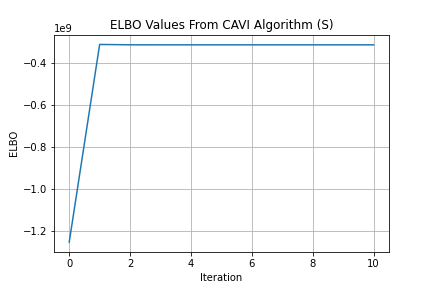
\includegraphics[width=\linewidth]{plots/ELBO_Values_From_CAVI_Algorithm_(S).png}
    \end{subfigure}
    \begin{subfigure}{0.32\textwidth}
        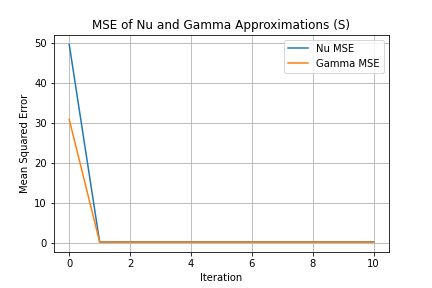
\includegraphics[width=\linewidth]{plots/MSE_of_Nu_and_Gamma_Approximations_(S).png}
    \end{subfigure}
    \begin{subfigure}{0.32\textwidth}
        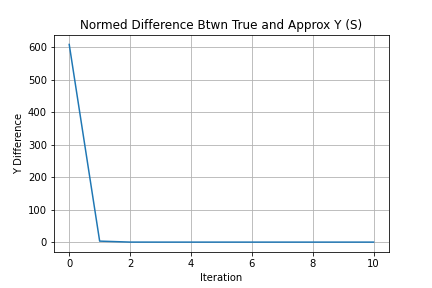
\includegraphics[width=\linewidth]{plots/Normed_Difference_Btwn_True_and_Approx_Y_(S).png}
    \end{subfigure}
    \caption{Plots for Specified Model: ELBO, MSE, and Norm Difference}
\end{figure}

\begin{figure}[h]
\centering
    \begin{subfigure}{0.32\textwidth}
        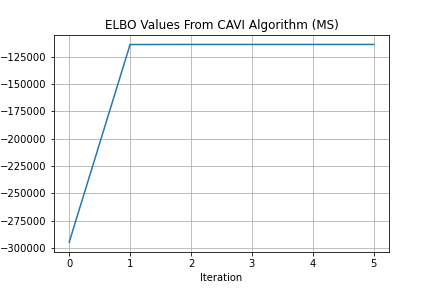
\includegraphics[width=\linewidth]{plots/ELBO_Values_From_CAVI_Algorithm_(MS).png}
    \end{subfigure}
    \begin{subfigure}{0.32\textwidth}
        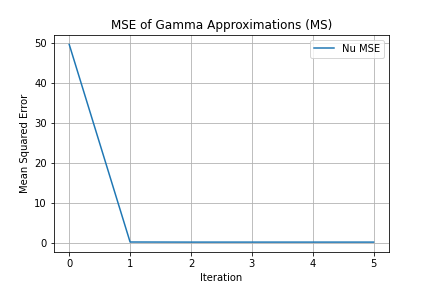
\includegraphics[width=\linewidth]{plots/MSE_of_Nu_Approximations_(MS).png}
    \end{subfigure}
    \begin{subfigure}{0.32\textwidth}
        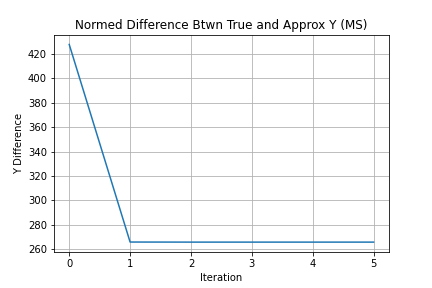
\includegraphics[width=\linewidth]{plots/Normed_Difference_Btwn_True_and_Approx_Y_(MS).png}
    \end{subfigure}
    \caption{Plots for Misspecified Model: ELBO, MSE, and Norm Difference}
\end{figure}

Then, I verify that for the regular posterior, misspecified variational approximations do worse than specified variational approximations. To do this, I (4) create a specified and misspecified linear model with the true latent variables and the approximated latent variables (both drawn from their respective priors) and plot them together. Notice how the specified model (S) is much more accurate than the misspecified model (MS).

\begin{figure}[h]
\centering
    \begin{subfigure}{0.49\textwidth}
        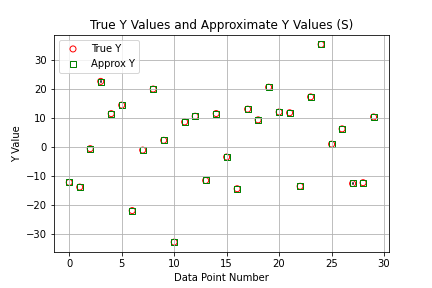
\includegraphics[width=\linewidth]{plots/True_Y_Values_and_Approximate_Y_Values_(S).png}
    \end{subfigure}
    \begin{subfigure}{0.49\textwidth}
        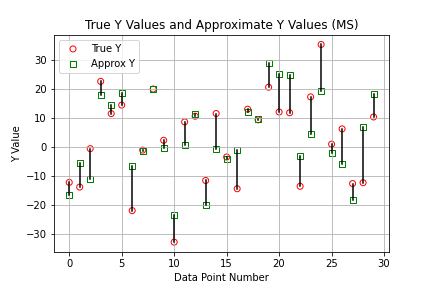
\includegraphics[width=\linewidth]{plots/True_Y_Values_and_Approximate_Y_Values_(MS).png}
    \end{subfigure}
    \caption{Comparing Linear Models and Approximate Linear Models in Specified and Misspecified Settings}
\end{figure}

These graphs simply verify that my models make sense. To show the robustness of variational approximations of $\alpha$ posteriors, I compute the KL-divergence from it to the true posterior. I do this for a variety of $\alpha$ values and pick the one that best minimizes the KL divergence. Finally, I compare the smallest KL-divergence -- from the best performing variational approximations of $\alpha$ posterior to the true posterior -- with the KL-divergence from the variational approximation of the posterior to the true posterior.

However, computing this proved more difficult than expected. Computing the true posterior $p(z|x)$ involves computing $p(x) = \int p(x|z)p(z) dz$ -- this is the exact intractable integral that motivated the use of VI in the first place. To examine VI's performance, I needed a different way to calculate $p(x)$. Scipy's integral solvers were unable to handle the high-dimensionality of $z$ so I turned to Markov Chain Monte Carlo (MCMC) estimates. However, like mentioned in the paper's introduction, MCMC is very time consuming and unfortunately, did not finish running before this paper's deadline. running.

\section{Conclusion}
Theoretical work has shown that in misspecified settings, $\alpha$-posteriors and their variational approximations are more robust than regular posteriors and their (respective) variational approximations. I seek to demonstrate this qualitatively. Although I constructed the variational approximations -- and have good reason to believe that they were successful -- I was ultimately unable to calculate the KL-divergence values necessary to prove this hypothesis. 

Computing KL-divergence efficiently in this type of setting is left for future work.

\section{Appendix A: Ideal CAVI Update for General Model}

Our goal is to find the ideal value for $q(z)$ that maximizes the ELBO. However, we approach this maximization problem one dimension at a time. Therefore, we actually want to find the ideal value for $q_j(z_j)$, chosen WLOG. This means that everything that is not dependent on $q_j(z_j)$ is treated as a constant and eventually dropped.

\begin{equation}
\begin{split}
    \elboq &= \E \el \log \pzx \er - \E \el \log \qz \er \\
    &= \int_z q(\z) \log \pzx d\z - \lb \mathbb{E}_{q_j} \el \log q_j(z_j) \er + \sum_{i \neq j} \mathbb{E}_{q_i} \el \log q_i(z_i) \er \rb \\ 
    &= \int_{z_j} q_j(z_j) \mathbb{E}_{q_{-j}} \el \log \pzx \er dz_j - \int_{z_j} q_j(z_j) \log q_j(z_j) dz_j + \textrm{const} \\
\end{split}
\end{equation}

Now let us define

\begin{equation}
    \log \tilde{p}_j(z_j, \x) =  \mathbb{E}_{q_{-j}} \el \log \pzx \er + \textrm{const}
\end{equation}

letting us write

\begin{equation}
\begin{split}
     \elboq &= \int_{z_j} q_j(z_j) \log \frac{\tilde{p}_j(z_j, \x)}{q_j(z_j)} dz_j + \textrm{const} \\
     &= - \kld{q_j(z_j)}{\tilde{p}_j(z_j, \x)} + \textrm{const}
\end{split}
\end{equation}

To maximize $\elboq$ with respect to a single $q_j(z_j)$, minimize KL. Because KL is non-negative, make it $0$ by setting $q_j(z_j) = \tilde{p}_j(z_j, \x)$. Our optimal value of $q_j(z_j)$ thus becomes

\begin{equation}
\begin{split}
    &q_j^*(z_j) = \tilde{p}_j(z_j, \x) = \exp \lc \mathbb{E}_{q_{-j}} \el \log \pzx \er \rc + \textrm{const}\\
    &\log q_j^*(z_j) \propto \mathbb{E}_{q_{-j}} \el \log \pzx \er
\end{split}
\end{equation}

\section{Appendix B: Ideal $\alpha$-CAVI Update for General Model}

Like in Appendix A, we want to find the value of $q(z)$ that maximizes the ELBO one dimension at a time. We follow the structure of Appendix A to find this ideal update.

\begin{equation}
\begin{split}
    \elbo_\alpha(q) &= \E \el \log \pz \er +  \E \el \log \pxgivenz^\alpha \er  - \E \el \log \qz \er\\
    &= \E \el \log \pz \pxgivenz^\alpha \er - \E \el \log \qz \er\\
    &= \int_z q(\z) \log \pz \pxgivenz^\alpha  d\z - \lb \mathbb{E}_{q_j} \el \log q_j(z_j) \er + \sum_{i \neq j} \mathbb{E}_{q_i} \el \log q_i(z_i) \er \rb \\ 
    &= \int_{z_j} q_j(\z_j) \mathbb{E}_{q_{-j}} \el \log \pz \pxgivenz^\alpha \er d\z_j -  \int_{z_j} q_j(\z_j) \log q_j(z_j) d\z_j + \textrm{const} \\ 
\end{split}
\end{equation}

Now let us define

\begin{equation}
    \log \tilde{p}_j(z_j, \x) =  \mathbb{E}_{q_{-j}} \el \log \pz \pxgivenz^\alpha \er + \textrm{const}
\end{equation}

letting us write

\begin{equation}
\begin{split}
     \textrm{ELBO}_\alpha(q) &= \int_{z_j} q_j(z_j) \log \frac{\tilde{p}_j(z_j, \x)}{q_j(z_j)} dz_j + \textrm{const} \\
     &= - \kld{q_j(z_j)}{\tilde{p}_j(z_j, \x)} + \textrm{const}
\end{split}
\end{equation}

Therefore, like in Appendix A, to maximize the $\alpha$-ELBO, set $q_j(z_j) = \tilde{p}_j(z_j, \x) $:

\begin{equation}
\begin{split}
    &q_j^*(z_j) = \tilde{p}_j(z_j, \x) = \exp \lc \mathbb{E}_{q_{-j}} \el \log \pz \pxgivenz^\alpha \er \rc + \textrm{const}\\
    &\log q_j^*(z_j) \propto \mathbb{E}_{q_{-j}} \el \log \pz \pxgivenz^\alpha \er
\end{split}
\end{equation}

    \section{Appendix C: Ideal $\alpha$-CAVI Update for Linear Model}

\subsection{Specified Model}

Recall that for a general model, the ideal parameter update is

\begin{equation}
    \log \qtheta \propto \Etheta \el \log \pz \pxgivenz^\alpha \er = \alpha \Etheta \el \log \pxgivenz \er +  \Etheta \el \log \pz \er
\end{equation}

For our specified model $y_i=\mathbf{\nu}^T\mathbf{t}_i+\mathbf{\gamma}^T \mathbf{r_i}+\epsilon_i$, this becomes:

\begin{equation}
    \log \qtheta \propto \alpha \Etheta \el \log p(\boldsymbol{y}|\nuv, \gammav) \er +  \Etheta \el \log p(\nuv, \gammav) \er
\end{equation}

We will simplify these expressions one at a time.
\\

\noindent \textbf{Expression 1:} We begin our calculations from the inside out, dropping any terms that are constant with respect to \nutheta

\begin{equation}
\begin{split}
    \log \pxgivenz &= \log \prod_i^n \pygiven\\
    &= \sum_i^n \log \lc (2\pi \sigmaepsilon )^{-\frac{1}{2}}  \exp \lp - \frac{\lp y_i - (\nuv^T \ti + \gammav^T \ri) \rp^2}{2 \sigmaepsilon} \rp \rc \\
    &= \sum_i^n \lb -\frac{1}{2} \log \lc 2\pi \sigmaepsilon \rc - \frac{\lp y_i - \nuv^T \ti - \gammav^T \ri \rp^2}{2 \sigmaepsilon} \rb \\
    &= - \frac{1}{2 \sigmaepsilon} \sum_i^n \lp y_i - \nuv^T \ti - \gammav \ri \rp ^2 + \text{const}
\end{split}
\end{equation}

Adding the rest of expression 1

\begin{equation}
\begin{split}
     \alpha \Etheta \el \log \pxgivenz \er &= -\frac{\alpha}{2 \sigmaepsilon} \sum_i^n \Etheta \lb \lp y_i - \nuv^T \ti - \gammav^T \ri \rp ^2  \rb  + \text{const}
\end{split}
\end{equation}

Now we focus on simplifying just the expectation. To simplify the notation, let and $\ytilde$, $\ttilde$, and $\rtilde$ represent an arbitrary $y_i$, $\ti$, and $\ri$ respectively. Again notice that we drop all terms that are constant with respect to \nutheta.

\begin{equation}
\begin{split}
    \Etheta & \lb \lp \ytilde - \nuv^T \ttilde - \gammav^T \rtilde \rp^2 \rb \\
    &= \Etheta \lb \ytilde^2 + \lp \nuv^T \ttilde \rp^2 + \lp \gammav^T \rtilde \rp^2 - 2 \ytilde \lp \nuv^T \ttilde \rp - 2 \ytilde \lp \gammav^T \rtilde \rp + 2 \lp \nuv^T \ttilde \rp \lp \gammav^T \rtilde \rp \rb \\
    &= \Etheta \lb \lp \nuv^T \ttilde \rp^2  - 2 \ytilde \lp \nuv^T \ttilde \rp  + 2 \lp \nuv^T \ttilde \rp \lp \gammav^T \rtilde \rp \rb + \text{const} \\
    &= \Etheta \lb \lp \nuv^T \ttilde \rp^2 \rb - \Etheta \lb  2 \ytilde \lp \nuv^T \ttilde \rp  \rb + \Etheta \lb 2 \lp \nuv^T \ttilde \rp \lp \gammav^T \rtilde \rp \rb + \text{const} 
\end{split}
\end{equation}

Furthermore, we handle the expectation terms one at at time. For the first expectation, we express our vector multiplication with a summation. We also take advantage of $\Sigmanu$, the covariance matrix of $\nuv$, which is defined only along its diagonals. This means that each element $\nuv_i$ is independent from $\nuv_j$ for all $i \neq j$. We can then use the independence properties of expectations to further simplify. Lastly, we also use the definition of variance $\text{Var}(x) = \mathbb{E}\lb x^2 \rb - \mathbb{E} \lb x \rb ^2$. 

\begin{equation}
\begin{split}
    \Etheta \lb \lp \sum_a \nua \tatilde \rp^2 \rb &= \Etheta \lb \sum_a  \lp \nua \tatilde \rp \sum_{a'} \lp \nuaprime \taprimetilde \rp \rb \\
    &= \sum_a \sum_{a'} \tatilde \taprimetilde \Etheta \lb \nua \nuaprime \rb \\
    &= \sum_a \lb \sum_{a' = a} \tatilde \taprimetilde \Etheta \lb \nua \nuaprime \rb + \sum_{a' \neq a} \tatilde \taprimetilde \Etheta \lb \nua \nuaprime \rb \rb \\
    &= \sum_a \tatilde^2 \Etheta \lb \nua^2 \rb + \sum_a \sum_{a' \neq a} \tatilde \taprimetilde \Etheta \lb \nua \rb \Etheta \lb \nuaprime \rb  \\
    &= \sum_{a=\theta} \tatilde^2 \lp \snusub{{a, a}} + \Etheta \lb \nua \rb^2 \rp \\
    & \qquad + \sum_{a=\theta} \sum_{a' \neq \theta} \tatilde \taprimetilde \Etheta \lb \nua \rb \Etheta \lb \nuaprime \rb\\
    & \qquad + \sum_{a \neq \theta} \sum_{a' = \theta} \tatilde \taprimetilde \Etheta \lb \nua \rb \Etheta \lb \nuaprime \rb  + \text{const} \\
    &= \tthetatilde^2 \lp \snusub{{\theta, \theta}} + \nutheta^2 \rp + \sum_{a' \neq \theta} \lp \tthetatilde \nutheta \rp \lp \tiaprime \mnusub{a'} \rp + \sum_{a \neq \theta} \lp \tthetatilde \nutheta \rp \lp \tia \mnusub{a} \rp + \text{const} \\
    &= \tthetatilde^2 \nutheta^2 + 2 \lp \tthetatilde \nutheta \rp \sum_{a \neq \theta} \lp \tia \mnusub{a} \rp + \text{const} \\
    &= \tthetatilde^2 \nutheta^2 + 2 \lp \tthetatilde \nutheta \rp \lp \sum_{a} \lp \tia \mnusub{a} \rp - \ti_\theta \mnusub{\theta}  \rp + \text{const} \\
    &= \tthetatilde^2 \nutheta^2 + 2 \lp \tthetatilde \nutheta \rp \lp {\mnu}^T \ti - \ti_\theta \mnusub{\theta}  \rp + \text{const} 
\end{split}
\end{equation}

Now we compute expectation 2

\begin{equation}
\begin{split}
    - \Etheta \lb 2 \ytilde \lp \sum_a \nua \tatilde \rp \rb &= -2 \ytilde \sum_a \tatilde \Etheta \lb \nua \rb \\
    &= -2 y_i \lp \tthetatilde \nutheta \rp + \text{const}
\end{split}
\end{equation}

Now we compute expectation 3

\begin{equation}
\begin{split}
    \Etheta \lb 2 \lp \sum_a \nua \tatilde \rp \lp \gammav^T \rtilde \rp \rb &= 2 \lp {\mgamma}^T \rtilde \rp \sum_a \tatilde \Etheta \lb \nua \rb \\
    &= 2 \lp {\mgamma}^T \ri \rp \lp \tthetatilde \nutheta \rp + \text{const} \\
\end{split}
\end{equation}

With these three expectations computed, we calculate all of expression 1, dropping the constants:

\begin{equation}
\begin{split}
    \alpha \Etheta \el \log \pxgivenz \er &= - \frac{\alpha}{2 \sigmaepsilon} \sum_{i=1}^n \lb \lc 2 \tthetatilde {\mgamma}^T \ri + 2 \tthetatilde \lp {\mnu}^T \ti - \mnusub{\theta} \ti_\theta \rp - 2 y_i \tthetatilde  \rc \nutheta + \lc \tthetatilde^2 \rc \nutheta^2  \rb \\
    &= \frac{\alpha}{ \sigmaepsilon} \sum_{i=1}^n \lb \bigg\{ y_i \tthetatilde - \tthetatilde {\mgamma}^T \ri - \tthetatilde {\mnu}^T \ti + \tthetatilde^2 \mnusub{\theta} \bigg\} \nutheta - \lc \frac{1}{2} \tthetatilde^2 \rc \nutheta^2  \rb \\
    &= \frac{\alpha}{ \sigmaepsilon} \sum_{i=1}^n \lb \bigg\{ \tthetatilde \lp y_i - {\mgamma}^T \ri - {\mnu}^T \ti + \mnusub{\theta} \tthetatilde \rp \bigg\} \nutheta - \lc \frac{1}{2} \tthetatilde^2 \rc \nutheta^2  \rb \\
    &= \lc  \frac{\alpha}{ \sigmaepsilon} \sum_{i=1}^n \tthetatilde \lp y_i - {\mgamma}^T \ri - {\mnu}^T \ti + \mnusub{\theta} \tthetatilde \rp \rc \nutheta - \lc \frac{\alpha}{2 \sigmaepsilon} \sum_{i=1}^n \tthetatilde^2 \rc \nutheta^2
\end{split}
\end{equation}

\noindent \textbf{Expression 2:} Now we calculate expression 2, again beginning from the inside and dropping all variables that are constant with respect to $\nutheta$

\begin{equation}
\begin{split}
    \log \pz &= \log p(\nuv) + \log p(\gammav) \\
    &= \log p(\nuv) + \text{const} \\
    &= \log \lc \lp 2 \pi \rp ^{-\frac{A}{2}} | \Sigmanu |^{-\frac{1}{2}} \exp \lp - \frac{1}{2} \lp \nuv - \meannu \rp^T \Sigmanu^{-1} \lp \nuv - \meannu \rp \rp \rc + \text{const} \\
    &= - \frac{1}{2} \lp \nuv - \meannu \rp^T \Sigmanu^{-1} \lp \nuv - \meannu \rp + \text{const}
\end{split}
\end{equation}

Adding in the rest of expression 2 and rewriting vector multiplication with summations:

\begin{equation}
\begin{split}
    \Etheta \el \log \pz \er &= \Etheta \el - \frac{1}{2} \lp \nuv - \meannu \rp^T \Sigmanu^{-1} \lp \nuv - \meannu \rp \er + \text{const} \\
    &= -\frac{1}{2} \Etheta \lb \sum_a \sum_{a'} \lp \nua - \meananu \rp \Sigmanu_{a,a'}^{-1} \lp \nuaprime - \meanaprimenu \rp \rb + \text{const} \\
    &= - \frac{1}{2} \sum_a \sum_{a'}  \Sigmanu_{a,a'}^{-1} \Etheta  \lb \lp \nua - \meananu \rp \lp \nuaprime - \meanaprimenu \rp \rb + \text{const} \\
    &= - \frac{1}{2} \sum_a \sum_{a'}  \Sigmanu_{a,a'}^{-1} \Etheta  \lb \nua \nuaprime - \meananu\nuaprime - \nua \meanaprimenu + \meananu \meanaprimenu \rb + \text{const} \\
\end{split}
\end{equation}

Now there are three terms that involve $\nutheta$, when $a=\theta$, $a' \neq \theta$, when $a \neq \theta$, $a' = \theta$, and when $a=\theta$, $a'=\theta$. The remaining summation terms are constants. Also note that because the precision matrix $\Sigmanu_{a,a'}^{-1}$ is defined as a diagonal matrix, it is zero everywhere off the diagonal.

\begin{equation}
\begin{split}
    & \quad - \frac{1}{2} \sum_{a=\theta} \sum_{a' \neq \theta}  \Sigmanu_{\theta,a'}^{-1} \Etheta  \lb \nutheta \nuaprime - \meannutheta \nuaprime - \nutheta \meanaprimenu + \meannutheta \meanaprimenu \rb \\
    &= - \frac{1}{2} \sum_{a' \neq \theta} 0 \cdot  \lp \nutheta \mnusub{a'} - \meannutheta \mnusub{a'} - \nutheta \meanaprimenu + \meannutheta \meanaprimenu \rp \\
    &= 0 + \textrm{const}
\end{split}
\end{equation}

Now by a symmetrical argument, the second term is:

\begin{equation}
\begin{split}
    & \quad - \frac{1}{2} \sum_{a \neq \theta} \sum_{a' = \theta}  \Sigmanu_{a,\theta}^{-1} \Etheta  \lb \nua \nutheta - \meananu\nutheta - \nua \meannutheta + \meananu \meannutheta \rb = 0 + \textrm{const}
\end{split}
\end{equation}

Finally, the third term is

\begin{equation}
\begin{split}
    & \quad - \frac{1}{2} \sum_{a=\theta} \sum_{a' = \theta}  \sigmanutheta^{-1} \Etheta  \lb \nutheta \nutheta - \meannutheta \nutheta - \nutheta \meannutheta + \meannutheta \meannutheta \rb \\
    &=  - \frac{1}{2}  \sigmanutheta^{-1} \lp \nutheta^2 - 2 \meannutheta \nutheta + \meannutheta^2 \rp \\
    &= - \frac{1}{2}  \sigmanutheta^{-1} \nutheta^2 + \sigmanutheta^{-1} \meannutheta \nutheta + \text{const}
\end{split}
\end{equation}

Now we compute the all of expression 2 and drop the constants.

\begin{equation}
\begin{split}
   \Etheta \el \log \pz \er &= \lc \sigmanutheta^{-1} \meannutheta \rc \nutheta - \lc \frac{1}{2} \sigmanutheta^{-1} \rc \nutheta^2
\end{split}
\end{equation}

\noindent \textbf{All Expressions Together:} Now we put expression 1 and expression 2 together, grouping terms according to their association with $\nutheta$ and $\nutheta^2$ respectively:

\begin{equation}
\begin{split}
    \log \qtheta &\propto \lc \sigmanutheta^{-1} \meannutheta + \frac{\alpha}{ \sigmaepsilon} \sum_{i=1}^n \tthetatilde \lp y_i - {\mgamma}^T \ri - {\mnu}^T \ti + \mnusub{\theta} \tthetatilde \rp \Bigg\} \nutheta - \lc \frac{1}{2} \sigmanutheta^{-1} + \frac{\alpha}{2 \sigmaepsilon} \sum_{i=1}^n  \tthetatilde^2 \rc \nutheta^2
\end{split}
\end{equation}

From this we find that the optimal variational density for $\log \qtheta$ is in the exponential family with sufficient statistics $\{ \nutheta,\nutheta^2\}$ and natural parameters $\{N_1,N_2\}$ of the form

\begin{equation}
\begin{split}
    \Bigg\{ \sigmanutheta^{-1} \meannutheta + &\frac{\alpha}{ \sigmaepsilon} \sum_{i=1}^n \tthetatilde \lp y_i - {\mgamma}^T \ri - {\mnu}^T \ti + \mnusub{\theta} \tthetatilde \rp , \quad - \frac{1}{2} \sigmanutheta^{-1} - \frac{\alpha}{2 \sigmaepsilon} \sum_{i=1}^n  \tthetatilde^2 \Bigg\}
\end{split}
\end{equation}

Therefore, the updates for the parameters of $\log \qtheta$ becomes:

\begin{equation}
\begin{split}
    s_{\nuv_{\theta, \theta}} &= - \frac{1}{2N_2} = \frac{1}{\sigmanutheta^{-1} + \frac{\alpha}{ \sigmaepsilon} \sum_{i=1}^n  \tthetatilde^2 }
\end{split}
\end{equation}

\begin{equation}
\begin{split}
    \mnusub{\theta} &= \frac{-N_1}{2N_2} = \frac{\sigmanutheta^{-1} \meannutheta + \frac{\alpha}{ \sigmaepsilon} \sum_{i=1}^n \tthetatilde \lp y_i - {\mgamma}^T \ri - {\mnu}^T \ti + \mnusub{\theta} \tthetatilde \rp }{ \sigmanutheta^{-1} + \frac{\alpha}{ \sigmaepsilon} \sum_{i=1}^n \tthetatilde^2 }\\
\end{split}
\end{equation}

We use a similar process to calculate $\log q(\gammav_\theta)$

\begin{equation}
\begin{split}
     \log \qgammatheta &\propto  \lc \Sigma_{\gammav_{\theta, \theta}}^{-1} \meangammatheta + \frac{\alpha}{ \sigmaepsilon} \sum_{i=1}^n \rvec{i_\theta} \lp y_i - {\mnu}^T \ti - {\mgamma}^T \ri + \mgammasub{\theta} \rvec{i_\theta} \rp \Bigg\} \gammav_\theta - \lc \frac{1}{2}  \Sigma_{\gammav_{\theta, \theta}}^{-1} + \frac{\alpha}{2 \sigmaepsilon} \sum_{i=1}^n \rvec{i_\theta}^2 \rc \gammav_\theta^2
\end{split}
\end{equation}

which again confirms that the optimal variational density for $\log \q(\gammav_\theta)$ is in the exponential family with sufficient statistics $\{ \gammav_\theta,\gammav_\theta^2\}$ and natural parameters $\{N_1,N_2\}$ of the form

\begin{equation}
\begin{split}
    \Bigg\{ \Sigma_{\gammav_{\theta, \theta}}^{-1} \meangammatheta + \frac{\alpha}{ \sigmaepsilon} \sum_{i=1}^n \rvec{i_\theta} \lp y_i - {\mnu}^T \ti - {\mgamma}^T \ri + \mgammasub{\theta} \rvec{i_\theta} \rp, \quad - \frac{1}{2} \Sigma_{\gammav_{\theta, \theta}}^{-1} - \frac{\alpha}{2 \sigmaepsilon} \sum_i^n \rvec{i_\theta}^2 \Bigg\}
\end{split}
\end{equation}

This gives us our ideal update equations for our variational densities

\begin{equation}
    s_{\gammav_{\theta, \theta}} = -\frac{1}{2 N_2}= \frac{1}{\Sigma_{\gammav_{\theta, \theta}}^{-1} + \frac{\alpha}{ \sigmaepsilon} \sum_{i=1}^n \rvec{i_\theta}^2 }
\end{equation}

\begin{equation}
    \mgammasub{\theta} = \frac{-N_1}{2N_2} = \frac{\Sigma_{\gammav_{\theta, \theta}}^{-1} \meangammatheta + \frac{\alpha}{ \sigmaepsilon} \sum_{i=1}^n \rvec{i_\theta} \lp y_i - {\mnu}^T \ti - {\mgamma}^T \ri + \mgammasub{\theta} \rvec{i_\theta} \rp}{\Sigma_{\gammav_{\theta, \theta}}^{-1} + \frac{\alpha}{ \sigmaepsilon} \sum_{i=1}^n \rvec{i_\theta}^2 }
\end{equation}
\\ \\
\noindent \textbf{Simplifying Constant Covariance Approximations $s_\nuv$ and $s_\gammav$:} Notice that the terms that appear in the covariance approximations $s_\nuv$ and $s_\gammav$ are all constant. This is an incredibly surprising result since once would assume that a good latent approximation $q(z)$ would update both its mean and covariance values. Here, updating the mean alone seems to get the job done. Further investigation is needed to determine exactly why this is so.

Therefore, we can calculate $s_\nuv$ and $s_\gammav$ once and then leave them unchanged -- this is reflected in the algorithm.

Additionally, because $s_\nuv$ and $s_\gammav$ are constant, we can simplify  $\elbo_\alpha$. We only care about the difference between $\elbo_\alpha$ iterations so if terms are otherwise constant with respect to $s_\nuv$ and $s_\gammav$, we drop them.

\subsection{Misspecified Model}
Recall that for a general model, the ideal parameter update is

\begin{equation}
    \log \qtheta \propto \Etheta \el \log \pz \pxgivenz^\alpha \er = \alpha \Etheta \el \log \pxgivenz \er +  \Etheta \el \log \pz \er
\end{equation}

For our misspecified model $y_i=\mathbf{\nu}^T\mathbf{t}_i+\epsilon_i$, this becomes:

\begin{equation}
    \log \qtheta \propto \alpha \Etheta \el \log p(\boldsymbol{y}|\nuv) \er +  \Etheta \el \log p(\nuv) \er
\end{equation}

We will simplify these expressions one at a time.
\\

\noindent \textbf{Expression 1:} We begin our calculations from the inside out, dropping any terms that are constant with respect to \nutheta

\begin{equation}
\begin{split}
    \log \pxgivenz &= \log \prod_i^n p(y_i|\nuv) \\
    &= \sum_i^n \log \lc (2\pi \sigmaepsilon )^{-\frac{1}{2}}  \exp \lp - \frac{\lp y_i - \nuv^T \ti \rp^2}{2 \sigmaepsilon} \rp \rc \\
    &= \sum_i^n \lb -\frac{1}{2} \log \lc 2\pi \sigmaepsilon \rc - \frac{\lp y_i - \nuv^T \ti \rp^2}{2 \sigmaepsilon} \rb \\
    &= - \frac{1}{2 \sigmaepsilon} \sum_i^n \lp y_i - \nuv^T \ti \rp ^2 + \text{const}
\end{split}
\end{equation}

Adding the rest of expression 1

\begin{equation}
\begin{split}
     \alpha \Etheta \el \log \pxgivenz \er &= -\frac{\alpha}{2 \sigmaepsilon} \sum_i^n \Etheta \lb \lp y_i - \nuv^T \ti \rp ^2  \rb  + \text{const}
\end{split}
\end{equation}

Now we focus on simplifying just the expectation. To simplify the notation, let and $\ytilde$, $\ttilde$, and $\rtilde$ represent an arbitrary $y_i$, $\ti$, and $\ri$ respectively.

\begin{equation}
\begin{split}
    \Etheta \lb \lp \ytilde - \nuv^T \ttilde \rp^2 \rb &= \Etheta \lb \ytilde^2 - 2 \ytilde \lp \nuv^T \ttilde \rp + \lp \nuv^T \ttilde \rp^2  \rb \\
    &= \Etheta \lb  \ytilde^2 \rb  - \Etheta \lb  2 \ytilde \lp \nuv^T \ttilde \rp  \rb + \Etheta \lb \lp \nuv^T \ttilde \rp^2 \rb \\
    &= \Etheta \lb \lp \nuv^T \ttilde \rp^2 \rb - \Etheta \lb  2 \ytilde \lp \nuv^T \ttilde \rp  \rb + \textrm{const}
\end{split}
\end{equation}

For the first expectation, we express our vector multiplication with a summation. We also take advantage of $\Sigmanu$, the covariance matrix of $\nuv$, which is defined only along its diagonals. This means that each element $\nuv_i$ is independent from $\nuv_j$ for all $i \neq j$. We can then use the independence properties of expectations to further simplify. Lastly, we also use the definition of variance $\text{Var}(x) = \mathbb{E}\lb x^2 \rb - \mathbb{E} \lb x \rb ^2$. 

\begin{equation}
\begin{split}
    \Etheta \lb \lp \sum_a \nua \tatilde \rp^2 \rb &= \Etheta \lb \sum_a  \lp \nua \tatilde \rp \sum_{a'} \lp \nuaprime \taprimetilde \rp \rb \\
    &= \sum_a \sum_{a'} \tatilde \taprimetilde \Etheta \lb \nua \nuaprime \rb \\
    &= \sum_a \lb \sum_{a' = a} \tatilde \taprimetilde \Etheta \lb \nua \nuaprime \rb + \sum_{a' \neq a} \tatilde \taprimetilde \Etheta \lb \nua \nuaprime \rb \rb \\
    &= \sum_a \tatilde^2 \Etheta \lb \nua^2 \rb + \sum_a \sum_{a' \neq a} \tatilde \taprimetilde \Etheta \lb \nua \rb \Etheta \lb \nuaprime \rb  \\
    &= \sum_{a=\theta} \tatilde^2 \lp \snusub{{a, a}} + \Etheta \lb \nua \rb^2 \rp \\
    & \qquad + \sum_{a=\theta} \sum_{a' \neq \theta} \tatilde \taprimetilde \Etheta \lb \nua \rb \Etheta \lb \nuaprime \rb\\
    & \qquad + \sum_{a \neq \theta} \sum_{a' = \theta} \tatilde \taprimetilde \Etheta \lb \nua \rb \Etheta \lb \nuaprime \rb  + \text{const} \\
    &= \tthetatilde^2 \lp \snusub{{\theta, \theta}} + \nutheta^2 \rp + \sum_{a' \neq \theta} \lp \tthetatilde \nutheta \rp \lp \tiaprime \mnusub{a'} \rp + \sum_{a \neq \theta} \lp \tthetatilde \nutheta \rp \lp \tia \mnusub{a} \rp + \text{const} \\
    &= \tthetatilde^2 \nutheta^2 + 2 \lp \tthetatilde \nutheta \rp \sum_{a \neq \theta} \lp \tia \mnusub{a} \rp + \text{const} \\
    &= \tthetatilde^2 \nutheta^2 + 2 \lp \tthetatilde \nutheta \rp \lp \sum_{a} \lp \tia \mnusub{a} \rp - \ti_\theta \mnusub{\theta}  \rp + \text{const} \\
    &= \tthetatilde^2 \nutheta^2 + 2 \lp \tthetatilde \nutheta \rp \lp {\mnu}^T \ti - \ti_\theta \mnusub{\theta}  \rp + \text{const} 
\end{split}
\end{equation}

Now we compute the 2nd expectation, dropping any terms that don't have to do with $\nuv_\theta$

\begin{equation}
\begin{split}
    - \Etheta \lb 2 \ytilde \lp \sum_a \nua \tatilde \rp \rb &= -2 \ytilde \sum_a \tatilde \Etheta \lb \nua \rb \\
    &= -2 y_i \lp \tthetatilde \nutheta \rp + \text{const}
\end{split}
\end{equation}

Now we calculate all of expression 1, dropping the constants:

\begin{equation}
\begin{split}
    \alpha \Etheta \el \log \pxgivenz \er &= - \frac{\alpha}{2 \sigmaepsilon} \sum_{i=1}^n \lb \lc 2 \tthetatilde \lp {\mnu}^T \ti - \mnusub{\theta} \ti_\theta \rp - 2 y_i \tthetatilde  \rc \nutheta + \lc \tthetatilde^2 \rc \nutheta^2  \rb \\
    &= \frac{\alpha}{ \sigmaepsilon} \sum_{i=1}^n \lb \bigg\{ y_i \tthetatilde - \tthetatilde {\mnu}^T \ti + \tthetatilde^2 \mnusub{\theta} \bigg\} \nutheta - \lc \frac{1}{2} \tthetatilde^2 \rc \nutheta^2  \rb \\
    &= \frac{\alpha}{ \sigmaepsilon} \sum_{i=1}^n \lb \bigg\{ \tthetatilde \lp y_i - {\mnu}^T \ti + \mnusub{\theta} \tthetatilde \rp \bigg\} \nutheta - \lc \frac{1}{2} \tthetatilde^2 \rc \nutheta^2  \rb \\
    &= \lc  \frac{\alpha}{ \sigmaepsilon} \sum_{i=1}^n \tthetatilde \lp y_i - {\mnu}^T \ti + \mnusub{\theta} \tthetatilde \rp \rc \nutheta - \lc \frac{\alpha}{2 \sigmaepsilon} \sum_{i=1}^n \tthetatilde^2 \rc \nutheta^2
\end{split}
\end{equation}

\noindent \textbf{Expression 2:} Now we calculate expression 2, again beginning from the inside and dropping all variables that are constant with respect to $\nutheta$

\begin{equation}
\begin{split}
    \log \pz &= \log p(\nuv) \\
    &= \log \lc \lp 2 \pi \rp ^{-\frac{A}{2}} | \Sigmanu |^{-\frac{1}{2}} \exp \lp - \frac{1}{2} \lp \nuv - \meannu \rp^T \Sigmanu^{-1} \lp \nuv - \meannu \rp \rp \rc \\
    &= - \frac{1}{2} \lp \nuv - \meannu \rp^T \Sigmanu^{-1} \lp \nuv - \meannu \rp + \text{const}
\end{split}
\end{equation}

Adding in the rest of expression 2 and rewriting vector multiplication with summations:

\begin{equation}
\begin{split}
    \Etheta \el \log \pz \er &= \Etheta \el - \frac{1}{2} \lp \nuv - \meannu \rp^T \Sigmanu^{-1} \lp \nuv - \meannu \rp \er + \text{const} \\
    &= -\frac{1}{2} \Etheta \lb \sum_a \sum_{a'} \lp \nua - \meananu \rp \Sigmanu_{a,a'}^{-1} \lp \nuaprime - \meanaprimenu \rp \rb + \text{const} \\
    &= - \frac{1}{2} \sum_a \sum_{a'}  \Sigmanu_{a,a'}^{-1} \Etheta  \lb \lp \nua - \meananu \rp \lp \nuaprime - \meanaprimenu \rp \rb + \text{const} \\
    &= - \frac{1}{2} \sum_a \sum_{a'}  \Sigmanu_{a,a'}^{-1} \Etheta  \lb \nua \nuaprime - \meananu\nuaprime - \nua \meanaprimenu + \meananu \meanaprimenu \rb + \text{const} \\
\end{split}
\end{equation}

Now there are three terms that involve $\nutheta$, when $a=\theta$, $a' \neq \theta$, when $a \neq \theta$, $a' = \theta$, and when $a=\theta$, $a'=\theta$. The remaining summation terms are constants. Also note that because the precision matrix $\Sigmanu_{a,a'}^{-1}$ is defined as a diagonal matrix, it is zero everywhere off the diagonal.

\begin{equation}
\begin{split}
    & \quad - \frac{1}{2} \sum_{a=\theta} \sum_{a' \neq \theta}  \Sigmanu_{\theta,a'}^{-1} \Etheta  \lb \nutheta \nuaprime - \meannutheta \nuaprime - \nutheta \meanaprimenu + \meannutheta \meanaprimenu \rb \\
    &= - \frac{1}{2} \sum_{a' \neq \theta} 0 \cdot  \lp \nutheta \mnusub{a'} - \meannutheta \mnusub{a'} - \nutheta \meanaprimenu + \meannutheta \meanaprimenu \rp \\
    &= 0 + \textrm{const}
\end{split}
\end{equation}

Now by a symmetrical argument, the second term is:

\begin{equation}
\begin{split}
    & \quad - \frac{1}{2} \sum_{a \neq \theta} \sum_{a' = \theta}  \Sigmanu_{a,\theta}^{-1} \Etheta  \lb \nua \nutheta - \meananu\nutheta - \nua \meannutheta + \meananu \meannutheta \rb = 0 + \textrm{const}
\end{split}
\end{equation}

Finally, the third term is

\begin{equation}
\begin{split}
    & \quad - \frac{1}{2} \sum_{a=\theta} \sum_{a' = \theta}  \sigmanutheta^{-1} \Etheta  \lb \nutheta \nutheta - \meannutheta \nutheta - \nutheta \meannutheta + \meannutheta \meannutheta \rb \\
    &=  - \frac{1}{2}  \sigmanutheta^{-1} \lp \nutheta^2 - 2 \meannutheta \nutheta + \meannutheta^2 \rp \\
    &= - \frac{1}{2}  \sigmanutheta^{-1} \nutheta^2 + \sigmanutheta^{-1} \meannutheta \nutheta + \text{const}
\end{split}
\end{equation}

Now we compute the all of expression 2 and drop the constants.


\begin{equation}
\begin{split}
   \Etheta \el \log \pz \er &= \lc \sigmanutheta^{-1} \meannutheta \rc \nutheta - \lc \frac{1}{2} \sigmanutheta^{-1} \rc \nutheta^2
\end{split}
\end{equation}

\noindent \textbf{All Expressions Together:} Now we put expression 1 and expression 2 together, grouping terms according to their association with $\nutheta$ and $\nutheta^2$ respectively:

\begin{equation}
\begin{split}
    \log \qtheta &\propto \lc \sigmanutheta^{-1} \meannutheta + \frac{\alpha}{ \sigmaepsilon} \sum_{i=1}^n \tthetatilde \lp y_i - {\mnu}^T \ti + \mnusub{\theta} \tthetatilde \rp \Bigg\} \nutheta - \lc \frac{1}{2} \sigmanutheta^{-1} + \frac{\alpha}{2 \sigmaepsilon} \sum_{i=1}^n  \tthetatilde^2 \rc \nutheta^2
\end{split}
\end{equation}

From this we find that the optimal variational density for $\log \qtheta$ is in the exponential family with sufficient statistics $\{ \nutheta,\nutheta^2\}$ and natural parameters $\{N_1,N_2\}$ of the form

\begin{equation}
\begin{split}
    \Bigg\{ \sigmanutheta^{-1} \meannutheta + &\frac{\alpha}{ \sigmaepsilon} \sum_{i=1}^n \tthetatilde \lp y_i - {\mnu}^T \ti + \mnusub{\theta} \tthetatilde \rp , \quad - \frac{1}{2} \sigmanutheta^{-1} - \frac{\alpha}{2 \sigmaepsilon} \sum_{i=1}^n  \tthetatilde^2 \Bigg\}
\end{split}
\end{equation}

Therefore, the updates for the parameters of $\log \qtheta$ becomes:

\begin{equation}
\begin{split}
    s_{\nuv_{\theta, \theta}} &= - \frac{1}{2N_2} = \frac{1}{\sigmanutheta^{-1} + \frac{\alpha}{ \sigmaepsilon} \sum_{i=1}^n  \tthetatilde^2 }
\end{split}
\end{equation}

\begin{equation}
\begin{split}
    \mnusub{\theta} &= \frac{-N_1}{2N_2} = \frac{\sigmanutheta^{-1} \meannutheta + \frac{\alpha}{ \sigmaepsilon} \sum_{i=1}^n \tthetatilde \lp y_i - {\mnu}^T \ti + \mnusub{\theta} \tthetatilde \rp }{ \sigmanutheta^{-1} + \frac{\alpha}{ \sigmaepsilon} \sum_{i=1}^n \tthetatilde^2 }\\
\end{split}
\end{equation}

\\ \\
\noindent \textbf{Simplifying Constant Covariance Approximations $s_\nuv$:} Once more, notice that the terms that appear in the covariance approximation $s_\nuv$ are constant. This is an incredibly surprising result since once would assume that a good latent approximation $q(z)$ would update both its mean and covariance values. Here, updating the mean alone seems to get the job done. Further investigation is needed to determine exactly why this is so.

Therefore, we can calculate $s_\nuv$ once and then leave it unchanged -- this is reflected in the algorithm.

Additionally, because $s_\nuv$ is constant, we can simplify  $\elbo_\alpha$. We only care about the difference between $\elbo_\alpha$ iterations so if terms are otherwise constant with respect to $s_\nuv$, we drop them.


\section{Appendix D: $\elbo_\alpha$ for Linear Model}

\subsection{Specified Model}

To check for convergence, we monitor the difference in the $\elbo_\alpha$ across iterations. To do this, we derive the $\elbo_\alpha$ equation for the specified model

\begin{equation}
    y_i=\mathbf{\nu}^T\mathbf{t}_i+\mathbf{\gamma}^T \mathbf{r_i}+\epsilon_i \qquad \text{for }i=1\ldots N 
\end{equation}

Recall the definition of the $\elbo_\alpha$:

\begin{equation}
\begin{split}
    \elbo_\alpha(q) &= \E \el \log \pxgivenz^\alpha \er + \E \el \log \pz \er   - \E \el \log \qz \er\\
    &= \alpha \E \lb \log p(\boldsymbol{y} | \nuv, \gammav) \rb + \E \lb \log p(\nuv) \rb + \E \lb \log p(\gammav) \rb - \E \lb \log q(\nuv) \rb - \E \lb \log q(\gammav) \rb \\
\end{split}
\end{equation}

We now simply these five expressions one by one

\textbf{Expression 1:}
\begin{equation}
\begin{split}
    \alpha \E \lb \log p(\boldsymbol{y} | \nuv, \gammav) \rb &= \alpha \E \lb \log \prod_{i=1}^n p(y_i | \nuv, \gammav) \rb \\
    &= \alpha \E \lb \sum \limits_{i=1}^N \log \lc (2 \pi \sigma_\epsilon^2)^{-\frac{1}{2}} \exp \left(- \frac{\left(y_i - \left(\nuv^T \ti + \gammav^T \ri \right) \right)^2}{2 \sigma_\epsilon^2} \right) \rc \rb \\
    &= -\frac{\alpha}{2 \sigmaepsilon} \sum_{i=1}^n \E \lb \lp y_i - \nuv^T \ti - \gammav^T \ri \rp^2 \rb + \textrm{const}
\end{split}
\end{equation}

Now we focus just on the expectation, rewriting $y_i$, $\ti$, and $\ri$ as $\ytilde$, $\ttilde$, and $\rtilde$ respectively. This allows us to simplify the notation.

\begin{equation}
\begin{split}
    \E \lb \lp \ytilde -\nuv^T \ttilde - \gammav^T \rtilde \rp ^2 \rb &= \E \lb \ytilde^2 \rb + \E \lb ( \nuv^T \ttilde)^2 \rb + \E \lb ( \gammav^T \rtilde)^2 \rb \\
    & \qquad - \E \lb 2 \ytilde \nuv^T \ttilde \rb - \E \lb 2 \ytilde \gammav^T \rtilde \rb + \E \lb 2 \nuv^T \ttilde \gammav^T \rtilde \rb \\
\end{split}
\end{equation}

Now we simplify each part of the expectation:

\begin{equation}
\begin{split}
     \E \lb \ytilde^2 \rb = \ytilde^2
\end{split}
\end{equation}

\begin{equation}
\begin{split}
    \E \lb ( \nuv^T \ttilde)^2 \rb &= \E \lb \lp \sum_a \nua \tatilde \rp \lp \sum_{a'} \nuaprime \taprimetilde \rp \rb \\
    &= \sum_a \sum_{a'} \tatilde \taprimetilde \E \lb \nua \nuaprime \rb \\
    &= \sum_a \lp \sum_{a' = a}  \tatilde \taprimetilde \E \lb \nua \nuaprime \rb + \sum_{a' \neq a}  \tatilde \taprimetilde \E \lb \nua \nuaprime \rb \rp \\
    &= \sum_a \lp \tatilde^2 \E \lb \nua ^2 \rb + \sum_{a' \neq a} \tatilde \taprimetilde \E \lb \nua \rb \E \lb \nuaprime \rb \rp \\
    &= \sum_a \tatilde^2 \lp s_{\nuv_{a,a}} + \mnusub{a}^2 \rp + \sum_a  \tatilde \mnusub{a} \sum_{a' \neq a} \taprimetilde \mnusub{a'} \\
    &= \sum_a \tatilde^2  s_{\nuv_{a,a}} + \sum_a \tatilde^2 \mnusub{a}^2 + \sum_a \tatilde \mnusub{a} \lp \ttilde^T {\mnu} - \tatilde \mnusub{a} \rp \\
    &= (\ttilde^2)^T ({\snu} \mathbb{I}) + (\ttilde^2)^T {\mnu}^2 + \ttilde^T   m_{\nuv} \sum_a \tatilde \mnusub{a} - \sum_a (\tatilde \mnusub{a} )^2 \\
    &= (\ttilde^2)^T ({\snu} \mathbb{I}) + (\ttilde^2)^T {\mnu}^2 + (\ttilde^T   m_{\nuv})^2  - (\ttilde^2)^T m_{\nuv}^2  \\
    &= (\ttilde^2)^T ({\snu} \mathbb{I}) + (\ttilde^T   m_{\nuv})^2 
\end{split}
\end{equation}

By similar argument:
\begin{equation}
\begin{split}
    \E \lb \lp \gammav^T \rtilde \rp ^2 \rb =  (\rtilde^2)^T ({\sgamma} \mathbb{I}) + (\rtilde^T   m_{\gammav})^2 
\end{split}
\end{equation}

\begin{equation}
\begin{split}
    - \E \lb 2 \ytilde \gammav^T \rtilde \rb &= -2 \ytilde \sum_b \E \lb \gammav_b \rb \rbtilde = -2 \ytilde {\mgamma}^T \rtilde
\end{split}
\end{equation}

\begin{equation}
\begin{split}
        - \E \lb 2 \ytilde \nuv^T \ttilde \rb = -2 \ytilde \sum_a \E \lb \nua \rb  \tatilde = - 2 \ytilde {\mnu}^T \ttilde 
\end{split}
\end{equation}

\begin{equation}
\begin{split}
    \E \lb 2 \nuv^T \ttilde \gammav^T \rtilde \rb &= 2 \sum_a \sum_b \E \lb \nua \rb  \tatilde \E \lb \gammav_b \rb \rbtilde = 2 \lp {\mnu}^T \ttilde \rp \lp {\mgamma}^T \rtilde \rp 
\end{split}
\end{equation}


Now we put all of expression one together, reverting back to the $i$ indexing notation.

\begin{equation}
\begin{split}
    \alpha \E \lb \log p(\boldsymbol{y} | \nuv, \gammav) \rb &= -\frac{\alpha}{2 \sigmaepsilon} \sum_{i=1}^n \Bigg[\ytilde^2 +  (\ti^2)^T ({\snu} \mathbb{I}) + (\ti^T   m_{\nuv})^2 + (\ri^2)^T ({\sgamma} \mathbb{I}) + (\ri^T   m_{\gammav})^2  \\
    & \qquad \qquad \qquad \quad -2 y_i {\mgamma}^T \ri - 2 y_i {\mnu}^T \ti + 2 \lp {\mnu}^T \ti \rp \lp {\mgamma}^T \ri \rp \Bigg] + \textrm{const} \\
    &= -\frac{\alpha}{2 \sigmaepsilon} \sum_{i=1}^n \Bigg[(y_i - \ti^T   m_{\nuv} - \ri^T   m_{\gammav})^2 \Bigg] -\frac{\alpha}{2 \sigmaepsilon} \sum_{i=1}^n \Bigg[ (\ti^2)^T ({\snu} \mathbb{I}) +  (\ri^2)^T ({\sgamma} \mathbb{I}) \Bigg] + \textrm{const} \\
\end{split}
\end{equation}

\textbf{Expression 2:}

\begin{equation}
\begin{split}
    \E \lb \log p(\nuv) \rb &= \E \lb \log \lc (2 \pi)^{-\frac{A}{2}}|\Sigmanu |^{-\frac{1}{2}} \exp \lp - \frac{1}{2} (\nuv - \mean{\nuv})^T \Sigmanu^{-1} (\nuv - \mean{\nuv}) \rp \rc \rb \\
    &= \E \lb - \frac{1}{2} (\nuv - \mean{\nuv})^T \Sigmanu^{-1} (\nuv - \mean{\nuv}) \rb + \textrm{const} \\
    &= - \frac{1}{2} \sum_a \sum_{a'}  \Sigmanu_{a,a'}^{-1} \E \lb \nua \nuaprime - \meananu \nuaprime - \meanaprimenu \nua + \meananu \meanaprimenu \rb + \textrm{const} \\
    &= - \frac{1}{2} \sum_a \lb \sum_{a'=a}  \Sigmanu_{a,a}^{-1} \E \lb \nua^2 - 2 \meananu \nua + \meananu^2 \rb \\
    & \qquad \qquad \qquad + \sum_{a' \neq a} \Sigmanu_{a,a'}^{-1} \E \lb  \nua \nuaprime - \meananu \nuaprime - \meanaprimenu \nua + \meananu \meanaprimenu \rb \Bigg] + \textrm{const} \\
    &= - \frac{1}{2} \sum_a \Bigg[  \Sigmanu_{a,a}^{-1} \lp \lp {\snu_{a,a}} + \mnusub{a}^2 \rp - 2 \meananu \mnusub{a} + \meananu^2 \rp \\
    & \qquad \qquad \qquad + \sum_{a' \neq a} \Sigmanu_{a,a'}^{-1} \lp \mnusub{a} \mnusub{a'} - \meananu \mnusub{a'} - \meanaprimenu \mnusub{a} + \meananu \meanaprimenu \rp \Bigg] + \textrm{const} \\
    &= - \frac{1}{2} \sum_a \Sigmanu_{a,a}^{-1} \lp {\snu_{a,a}} + \lp \mnusub{a} - \meananu \rp^2 \rp \\
    & \quad - \frac{1}{2} \sum_a \sum_{a' \neq a} \Sigmanu_{a,a'}^{-1} \lp  \mnusub{a}  - \meananu \rp \lp \mnusub{a'} - \meanaprimenu \rp  + \textrm{const} \\
    &= - \frac{1}{2} \sum_a \Sigmanu_{a,a}^{-1} \lp {\snu_{a,a}} + \lp \mnusub{a} - \meananu \rp^2 \rp \\
    & \quad - \frac{1}{2} \sum_a \bigg[ \sum_{a'} \Sigmanu_{a,a'}^{-1} \lp  \mnusub{a}  - \meananu \rp \lp \mnusub{a'} - \meanaprimenu \rp - \sum_{a'= a} \Sigmanu_{a,a}^{-1} \lp  \mnusub{a}  - \meananu \rp^2  \bigg]  + \textrm{const} \\
    &= - \frac{1}{2} \sum_a \Sigmanu_{a,a}^{-1} {\snu_{a,a}} - \frac{1}{2} \sum_a \Sigmanu_{a,a}^{-1} \lp \mnusub{a} - \meananu \rp^2 \\
    & \quad - \frac{1}{2} \sum_a \lp  \mnusub{a}  - \meananu \rp \sum_{a'} \Sigmanu_{a,a'}^{-1}  \lp \mnusub{a'} - \meanaprimenu \rp + \frac{1}{2} \sum_{a} \Sigmanu_{a,a}^{-1} \lp  \mnusub{a}  - \meananu \rp^2  + \textrm{const} \\
    & = - \frac{1}{2} \sum_a \Sigma_{\nuv_{a,a}}^{-1} {\snu_{a,a}} - \frac{1}{2} \sum_a \lp  \mnusub{a}  - \meananu \rp \sum_{a'} \Sigma_{\nuv_{a,a'}}^{-1}  \lp \mnusub{a'} - \meanaprimenu \rp \\
    &= - \frac{1}{2} (\Sigmanu^{-1} \mathbb{I} )^T (s_{\nuv} \mathbb{I}) - \frac{1}{2} (\Sigmanu^{-1} \mathbb{I} )^T \lp (m_{\nuv} - \boldsymbol{\mu}_{\nuv} )^2\rp + \textrm{const}
\end{split}
\end{equation}

\textbf{Expression 3:} We use a similar argument as Expression 2

\begin{equation}
\begin{split}
    \E \lb \log p(\gammav) \rb &= - \frac{1}{2} (\Sigmagamma^{-1} \mathbb{I} )^T (s_{\gammav} \mathbb{I}) - \frac{1}{2} (\Sigmagamma^{-1} \mathbb{I} )^T \lp (m_{\gammav} - \boldsymbol{\mu}_{\gammav} )^2\rp + \textrm{const}
\end{split}
\end{equation}

\textbf{Expression 4:}

\begin{equation}
\begin{split}
    - \E \lb \log q(\nuv) \rb &= -   \E \lb \log \lc (2 \pi)^{-\frac{A}{2}} | s_{\nuv} | ^{- \frac{1}{2}} \exp \lp - \frac{1}{2} (\nuv - {\mnu})^T s_{\nuv}^{-1} (\nuv - {\mnu})\rp \rc \rb \\
    &= -   \E \lb - \frac{1}{2} (\nuv - {\mnu})^T s_{\nuv}^{-1} (\nuv - {\mnu}) \rb + \textrm{const}\\
    &= - \frac{1}{2} \sum_a \sum_{a'} {\snu_{a,a'}}^{-1} \E \lb \nuv_a \nuv_{a'} - {\mnu_a} \nuv_{a'} - {\mnu_{a'}} \nuv_a + {\mnu_a} {\mnu_{a'}} \rb + \textrm{const} \\
    &= - \frac{1}{2} \sum_a \Bigg[ \sum_{a' = a}  {\snu_{a,a}}^{-1} \E \lb \nua^2 - 2 \mnusub{a} \nua + \mnusub{a}^2 \rb \\
    & \qquad \qquad \qquad + \sum_{a' \neq a}  {\snu_{a,a'}}^{-1} \E \lb \nuv_a \nuv_{a'} - {\mnu_a} \nuv_{a'} - {\mnu_{a'}} \nuv_a + {\mnu_a} {\mnu_{a'}} \rb \Bigg] + \textrm{const} \\
    &= - \frac{1}{2} \sum_a \Bigg[  {\snu_{a,a}}^{-1} \lp \lp {\snu_{a,a}} + \mnusub{a}^2\rp - 2 \mnusub{a}^2 + \mnusub{a}^2 \rp \\
    & \qquad \qquad \qquad + \sum_{a' \neq a}  {\snu_{a,a'}}^{-1} \lp \mnusub{a} \mnusub{a'} - \mnusub{a} \mnusub{a'} - \mnusub{a'} \mnusub{a} + \mnusub{a} \mnusub{a'}\rp \Bigg] + \textrm{const} \\
    &= - \frac{1}{2} \sum_a \Bigg[ {\snu_{a,a'}}^{-1} {\snu_{a,a'}} + {s_{\nuv}_{a,a'}}^{-1} \lp  \mnusub{a}^2 - 2 \mnusub{a}^2 + \mnusub{a}^2 \rp \Bigg] + \textrm{const} \\
    &= - \frac{1}{2} \sum_{a=1}^A {\snu_{a,a'}}^{-1} {\snu_{a,a'}} + \textrm{const} = - \frac{1}{2} \sum_{a=1}^A 1 + \textrm{const} \\
    &= - \frac{  A}{2} + \textrm{const} = \textrm{const}
\end{split}
\end{equation}


\textbf{Expression 5:}

By similar argument we conclude that: 

\begin{equation}
\begin{split}
    -   \E \lb \log q(\gammav) \rb &= \textrm{const}
\end{split}
\end{equation}

\textbf{All Expressions Together:} Now we put all expressions together to get our final $\elbo_\alpha$ equation. Note that we drop constants because we only care about the difference between $\elbo_\alpha$ values

\begin{equation}
\begin{split}
    \elbo_\alpha(q) &= -\frac{\alpha}{2 \sigmaepsilon} \sum_{i=1}^n \Bigg[(y_i - \ti^T   m_{\nuv} - \ri^T   m_{\gammav})^2 \Bigg] -\frac{\alpha}{2 \sigmaepsilon} \sum_{i=1}^n \Bigg[ (\ti^2)^T ({\snu} \mathbb{I}) +  (\ri^2)^T ({\sgamma} \mathbb{I}) \Bigg] \\
    & \quad - \frac{1}{2} \Bigg[ (\Sigmanu^{-1} \mathbb{I} )^T (s_{\nuv} \mathbb{I}) + (\Sigmanu^{-1} \mathbb{I} )^T (m_{\nuv}  - \boldsymbol{\mu}_{\nuv} )^2 + (\Sigmagamma^{-1} \mathbb{I} )^T (s_{\gammav} \mathbb{I}) + (\Sigmagamma^{-1} \mathbb{I} )^T (m_{\gammav} - \boldsymbol{\mu}_{\gammav} )^2\ \Bigg] \\
\end{split}
\end{equation}

\noindent \textbf{Simplifying With Constant $s_\nuv$ and $s_\gammav$:}

Because $s_\nuv$ and $s_\gammav$ are constant, we can take them out of our $\elbo_\alpha$ calculations. Our final equation then becomes: 

\begin{equation}
\begin{split}
    \elbo_\alpha(q) &= -\frac{\alpha}{2 \sigmaepsilon} \sum_{i=1}^n \Bigg[(y_i - \ti^T   m_{\nuv} - \ri^T   m_{\gammav})^2 \Bigg] - \frac{1}{2} \Bigg[ (\Sigmanu^{-1} \mathbb{I} )^T (m_{\nuv}  - \boldsymbol{\mu}_{\nuv} )^2 + (\Sigmagamma^{-1} \mathbb{I} )^T (m_{\gammav} - \boldsymbol{\mu}_{\gammav} )^2\ \Bigg] \\
\end{split}
\end{equation}

\subsection{Misspecified Model}

To check for convergence, we monitor the difference in the $\elbo_\alpha$ across iterations. To do this, we derive the $\elbo_\alpha$ equation for the misspecified model

\begin{equation}
    y_i=\mathbf{\nu}^T\mathbf{t}_i+\epsilon_i \qquad \text{for }i=1\ldots N 
\end{equation}

Recall the definition of the $\elbo_\alpha$:

\begin{equation}
\begin{split}
    \elbo_\alpha(q) &= \E \el \log \pxgivenz^\alpha \er + \E \el \log \pz \er   - \E \el \log \qz \er\\
    &= \alpha \E \lb \log p(\boldsymbol{y} | \nuv) \rb + \E \lb \log p(\nuv) \rb  - \E \lb \log q(\nuv) \rb \\
\end{split}
\end{equation}

We now simply these three expressions one by one

\textbf{Expression 1:}
\begin{equation}
\begin{split}
    \alpha \E \lb \log p(\boldsymbol{y} | \nuv) \rb &= \alpha \E \lb \log \prod_{i=1}^n p(y_i | \nuv) \rb \\
    &= \alpha \E \lb \sum \limits_{i=1}^N \log \lc (2 \pi \sigma_\epsilon^2)^{-\frac{1}{2}} \exp \left(- \frac{\left(y_i - \nuv^T \ti \right)^2}{2 \sigma_\epsilon^2} \right) \rc \rb \\
    &= -\frac{\alpha}{2 \sigmaepsilon} \sum_{i=1}^n \E \lb \lp y_i - \nuv^T \ti \rp^2 \rb + \textrm{const}
\end{split}
\end{equation}

Now we focus just on the expectation, rewriting $y_i$, $\ti$, and $\ri$ as $\ytilde$, $\ttilde$, and $\rtilde$ respectively. This allows us to simplify the notation.

\begin{equation}
\begin{split}
    \E \lb \lp \ytilde -\nuv^T \ttilde \rp ^2 \rb &= \E \lb \ytilde^2 \rb - \E \lb 2 \ytilde \nuv^T \ttilde \rb + \E \lb ( \nuv^T \ttilde)^2 \rb 
\end{split}
\end{equation}

Now we simplify each part of the expectation:

\begin{equation}
\begin{split}
     \E \lb \ytilde^2 \rb = \ytilde^2 
\end{split}
\end{equation}

\begin{equation}
\begin{split}
        - \E \lb 2 \ytilde \nuv^T \ttilde \rb = -2 \ytilde \sum_a \E \lb \nua \rb  \tatilde = - 2 \ytilde {\mnu}^T \ttilde 
\end{split}
\end{equation}

\begin{equation}
\begin{split}
    \E \lb ( \nuv^T \ttilde)^2 \rb &= \E \lb \lp \sum_a \nua \tatilde \rp \lp \sum_{a'} \nuaprime \taprimetilde \rp \rb \\
    &= \sum_a \sum_{a'} \tatilde \taprimetilde \E \lb \nua \nuaprime \rb \\
    &= \sum_a \lp \sum_{a' = a}  \tatilde \taprimetilde \E \lb \nua \nuaprime \rb + \sum_{a' \neq a}  \tatilde \taprimetilde \E \lb \nua \nuaprime \rb \rp \\
    &= \sum_a \lp \tatilde^2 \E \lb \nua ^2 \rb + \sum_{a' \neq a} \tatilde \taprimetilde \E \lb \nua \rb \E \lb \nuaprime \rb \rp \\
    &= \sum_a \tatilde^2 \lp s_{\nuv_{a,a}} + \mnusub{a}^2 \rp + \sum_a  \tatilde \mnusub{a} \sum_{a' \neq a} \taprimetilde \mnusub{a'} \\
    &= \sum_a \tatilde^2  s_{\nuv_{a,a}} + \sum_a \tatilde^2 \mnusub{a}^2 + \sum_a \tatilde \mnusub{a} \lp \ttilde^T {\mnu} - \tatilde \mnusub{a} \rp \\
    &= (\ttilde^2)^T ({\snu} \mathbb{I}) + (\ttilde^2)^T {\mnu}^2 + \ttilde^T   m_{\nuv} \sum_a \tatilde \mnusub{a} - \sum_a (\tatilde \mnusub{a} )^2 \\
    &= (\ttilde^2)^T ({\snu} \mathbb{I}) + (\ttilde^2)^T {\mnu}^2 + (\ttilde^T   m_{\nuv})^2  - (\ttilde^2)^T m_{\nuv}^2  \\
    &= (\ttilde^2)^T ({\snu} \mathbb{I}) + (\ttilde^T   m_{\nuv})^2 
\end{split}
\end{equation}

Now we put all of expression one together, reverting back to the $i$ indexing notation.

\begin{equation}
\begin{split}
    \alpha \E \lb \log p(\boldsymbol{y} | \nuv) \rb &= -\frac{\alpha}{2 \sigmaepsilon} \sum_{i=1}^n \Bigg[\ytilde^2 + (\ti^2)^T ({\snu} \mathbb{I}) + (\ti^T   m_{\nuv})^2  - 2 y_i {\mnu}^T \ti \Bigg] + \textrm{const} \\
    &= -\frac{\alpha}{2 \sigmaepsilon} \sum_{i=1}^n \Bigg[(y_i - {\mnu}^T \ti)^2 \Bigg] -\frac{\alpha}{2 \sigmaepsilon} \sum_{i=1}^n \Bigg[ (\ti^2)^T ({\snu} \mathbb{I}) \Bigg] + \textrm{const} \\
\end{split}
\end{equation}

\textbf{Expression 2:}

\begin{equation}
\begin{split}
    \E \lb \log p(\nuv) \rb &= \E \lb \log \lc (2 \pi)^{-\frac{A}{2}}|\Sigmanu |^{-\frac{1}{2}} \exp \lp - \frac{1}{2} (\nuv - \mean{\nuv})^T \Sigmanu^{-1} (\nuv - \mean{\nuv}) \rp \rc \rb \\
    &= \E \lb - \frac{1}{2} (\nuv - \mean{\nuv})^T \Sigmanu^{-1} (\nuv - \mean{\nuv}) \rb + \textrm{const} \\
    &= - \frac{1}{2} \sum_a \sum_{a'}  \Sigmanu_{a,a'}^{-1} \E \lb \nua \nuaprime - \meananu \nuaprime - \meanaprimenu \nua + \meananu \meanaprimenu \rb + \textrm{const} \\
    &= - \frac{1}{2} \sum_a \lb \sum_{a'=a}  \Sigmanu_{a,a}^{-1} \E \lb \nua^2 - 2 \meananu \nua + \meananu^2 \rb \\
    & \qquad \qquad \qquad + \sum_{a' \neq a} \Sigmanu_{a,a'}^{-1} \E \lb  \nua \nuaprime - \meananu \nuaprime - \meanaprimenu \nua + \meananu \meanaprimenu \rb \Bigg] + \textrm{const} \\
    &= - \frac{1}{2} \sum_a \Bigg[  \Sigmanu_{a,a}^{-1} \lp \lp {\snu_{a,a}} + \mnusub{a}^2 \rp - 2 \meananu \mnusub{a} + \meananu^2 \rp \\
    & \qquad \qquad \qquad + \sum_{a' \neq a} \Sigmanu_{a,a'}^{-1} \lp \mnusub{a} \mnusub{a'} - \meananu \mnusub{a'} - \meanaprimenu \mnusub{a} + \meananu \meanaprimenu \rp \Bigg] + \textrm{const} \\
    &= - \frac{1}{2} \sum_a \Sigmanu_{a,a}^{-1} \lp {\snu_{a,a}} + \lp \mnusub{a} - \meananu \rp^2 \rp \\
    & \quad - \frac{1}{2} \sum_a \sum_{a' \neq a} \Sigmanu_{a,a'}^{-1} \lp  \mnusub{a}  - \meananu \rp \lp \mnusub{a'} - \meanaprimenu \rp  + \textrm{const} \\
    &= - \frac{1}{2} \sum_a \Sigmanu_{a,a}^{-1} \lp {\snu_{a,a}} + \lp \mnusub{a} - \meananu \rp^2 \rp \\
    & \quad - \frac{1}{2} \sum_a \bigg[ \sum_{a'} \Sigmanu_{a,a'}^{-1} \lp  \mnusub{a}  - \meananu \rp \lp \mnusub{a'} - \meanaprimenu \rp - \sum_{a'= a} \Sigmanu_{a,a}^{-1} \lp  \mnusub{a}  - \meananu \rp^2  \bigg]  + \textrm{const} \\
    &= - \frac{1}{2} \sum_a \Sigmanu_{a,a}^{-1} {\snu_{a,a}} - \frac{1}{2} \sum_a \Sigmanu_{a,a}^{-1} \lp \mnusub{a} - \meananu \rp^2 \\
    & \quad - \frac{1}{2} \sum_a \lp  \mnusub{a}  - \meananu \rp \sum_{a'} \Sigmanu_{a,a'}^{-1}  \lp \mnusub{a'} - \meanaprimenu \rp + \frac{1}{2} \sum_{a} \Sigmanu_{a,a}^{-1} \lp  \mnusub{a}  - \meananu \rp^2  + \textrm{const} \\
    & = - \frac{1}{2} \sum_a \Sigma_{\nuv_{a,a}}^{-1} {\snu_{a,a}} - \frac{1}{2} \sum_a \lp  \mnusub{a}  - \meananu \rp \sum_{a'} \Sigma_{\nuv_{a,a'}}^{-1}  \lp \mnusub{a'} - \meanaprimenu \rp \\
    &= - \frac{1}{2} (\Sigmanu^{-1} \mathbb{I} )^T (s_{\nuv} \mathbb{I}) - \frac{1}{2} (\Sigmanu^{-1} \mathbb{I} )^T \lp (m_{\nuv} - \boldsymbol{\mu}_{\nuv} )^2\rp + \textrm{const}
\end{split}
\end{equation}

\textbf{Expression 3:}

\begin{equation}
\begin{split}
    - \E \lb \log q(\nuv) \rb &= -   \E \lb \log \lc (2 \pi)^{-\frac{A}{2}} | s_{\nuv} | ^{- \frac{1}{2}} \exp \lp - \frac{1}{2} (\nuv - {\mnu})^T s_{\nuv}^{-1} (\nuv - {\mnu})\rp \rc \rb \\
    &= -   \E \lb - \frac{1}{2} (\nuv - {\mnu})^T s_{\nuv}^{-1} (\nuv - {\mnu}) \rb + \textrm{const}\\
    &= - \frac{1}{2} \sum_a \sum_{a'} {\snu_{a,a'}}^{-1} \E \lb \nuv_a \nuv_{a'} - {\mnu_a} \nuv_{a'} - {\mnu_{a'}} \nuv_a + {\mnu_a} {\mnu_{a'}} \rb + \textrm{const} \\
    &= - \frac{1}{2} \sum_a \Bigg[ \sum_{a' = a}  {\snu_{a,a}}^{-1} \E \lb \nua^2 - 2 \mnusub{a} \nua + \mnusub{a}^2 \rb \\
    & \qquad \qquad \qquad + \sum_{a' \neq a}  {\snu_{a,a'}}^{-1} \E \lb \nuv_a \nuv_{a'} - {\mnu_a} \nuv_{a'} - {\mnu_{a'}} \nuv_a + {\mnu_a} {\mnu_{a'}} \rb \Bigg] + \textrm{const} \\
    &= - \frac{1}{2} \sum_a \Bigg[  {\snu_{a,a}}^{-1} \lp \lp {\snu_{a,a}} + \mnusub{a}^2\rp - 2 \mnusub{a}^2 + \mnusub{a}^2 \rp \\
    & \qquad \qquad \qquad + \sum_{a' \neq a}  {\snu_{a,a'}}^{-1} \lp \mnusub{a} \mnusub{a'} - \mnusub{a} \mnusub{a'} - \mnusub{a'} \mnusub{a} + \mnusub{a} \mnusub{a'}\rp \Bigg] + \textrm{const} \\
    &= - \frac{1}{2} \sum_a \Bigg[ {\snu_{a,a'}}^{-1} {\snu_{a,a'}} + {s_{\nuv}_{a,a'}}^{-1} \lp  \mnusub{a}^2 - 2 \mnusub{a}^2 + \mnusub{a}^2 \rp \Bigg] + \textrm{const} \\
    &= - \frac{1}{2} \sum_{a=1}^A {\snu_{a,a'}}^{-1} {\snu_{a,a'}} + \textrm{const} = - \frac{1}{2} \sum_{a=1}^A 1 + \textrm{const} \\
    &= - \frac{  A}{2} + \textrm{const} = \textrm{const}
\end{split}
\end{equation}


\textbf{All Expressions Together:} Now we put all expressions together to get $\elbo_\alpha$ equation. Note that we drop constants because we only care about the difference between $\elbo_\alpha$ values

\begin{equation}
\begin{split}
    \elbo_\alpha(q) &= -\frac{\alpha}{2 \sigmaepsilon} \sum_{i=1}^n \Bigg[(y_i - {\mnu}^T \ti)^2 \Bigg] -\frac{\alpha}{2 \sigmaepsilon} \sum_{i=1}^n \Bigg[ (\ti^2)^T ({\snu} \mathbb{I}) \Bigg] \\
    & \quad - \frac{1}{2} \Bigg[ (\Sigmanu^{-1} \mathbb{I} )^T (s_{\nuv} \mathbb{I}) + (\Sigmanu^{-1} \mathbb{I} )^T (m_{\nuv}  - \boldsymbol{\mu}_{\nuv} )^2 \Bigg] \\
\end{split}
\end{equation}

\noindent \textbf{Simplifying With Constant $s_\nuv$:}

Because $s_\nuv$ is constant, we can take them out of our $\elbo_\alpha$ calculations. Our final equation then becomes: 

\begin{equation}
\begin{split}
    \elbo_\alpha(q) &= -\frac{\alpha}{2 \sigmaepsilon} \sum_{i=1}^n \Bigg[(y_i - {\mnu}^T \ti)^2 \Bigg] - \frac{1}{2} (\Sigmanu^{-1} \mathbb{I} )^T (m_{\nuv}  - \boldsymbol{\mu}_{\nuv} )^2 \\
\end{split}
\end{equation}

\printbibliography

\end{document}
